% Für Bindekorrektur als optionales Argument "BCORfaktormitmaßeinheit", dann
% sieht auch Option "twoside" vernünftig aus
% Näheres zu "scrartcl" bzw. "scrreprt" und "scrbook" siehe KOMA-Skript Doku
\documentclass[12pt,a4paper,titlepage,headinclude,bibtotoc]{scrartcl}


%---- Allgemeine Layout Einstellungen ------------------------------------------

% Für Kopf und Fußzeilen, siehe auch KOMA-Skript Doku
\usepackage[komastyle]{scrpage2}
\pagestyle{scrheadings}
\automark[section]{chapter}
\setheadsepline{0.5pt}[\color{black}]

%keine Einrückung
\parindent0pt

%Einstellungen für Figuren- und Tabellenbeschriftungen
\setkomafont{captionlabel}{\sffamily\bfseries}
\setcapindent{0em}

\usepackage{caption}

%---- Weitere Pakete -----------------------------------------------------------
% Die Pakete sind alle in der TeX Live Distribution enthalten. Wichtige Adressen
% www.ctan.org, www.dante.de

% Sprachunterstützung
\usepackage[ngerman]{babel}

% Benutzung von Umlauten direkt im Text
% entweder "latin1" oder "utf8"
\usepackage[utf8]{inputenc}

% Pakete mit Mathesymbolen und zur Beseitigung von Schwächen der Mathe-Umgebung
\usepackage{latexsym,exscale,amssymb,amsmath}

% Weitere Symbole
\usepackage[nointegrals]{wasysym}
\usepackage{eurosym}

% Anderes Literaturverzeichnisformat
%\usepackage[square,sort&compress]{natbib}

% Für Farbe
\usepackage{color}

% Zur Graphikausgabe
%Beipiel: \includegraphics[width=\textwidth]{grafik.png}
\usepackage{graphicx}

% Text umfließt Graphiken und Tabellen
% Beispiel:
% \begin{wrapfigure}[Zeilenanzahl]{"l" oder "r"}{breite}
%   \centering
%   \includegraphics[width=...]{grafik}
%   \caption{Beschriftung} 
%   \label{fig:grafik}
% \end{wrapfigure}
\usepackage{wrapfig}

% Mehrere Abbildungen nebeneinander
% Beispiel:
% \begin{figure}[htb]
%   \centering
%   \subfigure[Beschriftung 1\label{fig:label1}]
%   {\includegraphics[width=0.49\textwidth]{grafik1}}
%   \hfill
%   \subfigure[Beschriftung 2\label{fig:label2}]
%   {\includegraphics[width=0.49\textwidth]{grafik2}}
%   \caption{Beschriftung allgemein}
%   \label{fig:label-gesamt}
% \end{figure}
\usepackage{subfigure}
\usepackage{adjustbox}

% Caption neben Abbildung
% Beispiel:
% \sidecaptionvpos{figure}{"c" oder "t" oder "b"}
% \begin{SCfigure}[rel. Breite (normalerweise = 1)][hbt]
%   \centering
%   \includegraphics[width=0.5\textwidth]{grafik.png}
%   \caption{Beschreibung}
%   \label{fig:}
% \end{SCfigure}
\usepackage{sidecap}

% Befehl für "Entspricht"-Zeichen
\newcommand{\corresponds}{\ensuremath{\mathrel{\widehat{=}}}}

%Für chemische Formeln (von www.dante.de)
%% Anpassung an LaTeX(2e) von Bernd Raichle
\makeatletter
\DeclareRobustCommand{\chemical}[1]{%
  {\(\m@th
   \edef\resetfontdimens{\noexpand\)%
       \fontdimen16\textfont2=\the\fontdimen16\textfont2
       \fontdimen17\textfont2=\the\fontdimen17\textfont2\relax}%
   \fontdimen16\textfont2=2.7pt \fontdimen17\textfont2=2.7pt
   \mathrm{#1}%
   \resetfontdimens}}
\makeatother

%Si Einheiten
\usepackage{siunitx}

%c++ Code einbinden
\usepackage{listings}
\lstset{numbers=left, numberstyle=\tiny, numbersep=5pt}

%Differential
\newcommand{\dif}{\ensuremath{\mathrm{d}}}
%sinc
\newcommand{\sinc}{\ensuremath{\mathrm{sinc}}}

%Boxen,etc.
\usepackage{fancybox}
\usepackage{empheq}

%Fußnoten auf gleiche Seite
\interfootnotelinepenalty=1000

%Dateien aus Unterverzeichnissen
\usepackage{import}

%Bibliography \bibliography{literatur} und \cite{gerthsen}
%\usepackage{cite}
\usepackage{babelbib}
\selectbiblanguage{ngerman}

\begin{document}

\begin{titlepage}
\centering
\textsc{\Large Anfängerpraktikum der Fakultät für
  Physik,\\[1.5ex] Universität Göttingen}

\vspace*{4.2cm}

\rule{\textwidth}{1pt}\\[0.5cm]
{\huge \bfseries
  Beugung und Interferenz\\[1.5ex]
  von Laserlicht}\\[0.5cm]
\rule{\textwidth}{1pt}

\vspace*{3.0cm}

\begin{Large}
\begin{tabular}{ll}
Praktikant:
 	&  Felix Kurtz\\
 	&  Michael Lohmann\\

E-Mail: 
	&  felix.kurtz@stud.uni-goettingen.de\\
	& m.lohmann@stud.uni-goettingen.de\\

 Betreuer: & Phillip Bastian\\
 Versuchsdatum: &  09.03.2015\\
\end{tabular}
\end{Large}

\vspace*{0.8cm}

\begin{Large}
\fbox{
  \begin{minipage}[t][2.5cm][t]{6cm} 
    Testat:
  \end{minipage}
}
\end{Large}

\end{titlepage}

\tableofcontents

\newpage

\section{Einleitung}
\label{sec:einleitung}
In diesem Versuch sollen die Eigenschaften von Laserlicht für Beugung und Interferenz an verschiedenen Objekten genutzt werden.
Da ein Laser auf stimulierter Emission von Photonen basiert, ist sein Licht nämlich sehr monochromatisch sowie zeitlich und räumlich kohärent.
Als Lichtquelle wird diesmal ein Helium-Neon-Laser verwendet, der Intensitätsverlauf wird über eine mit einem Schrittmotor bewegbare Fotodiode elektronisch aufgenommen.

\section{Theorie}
\label{sec:theorie}
\subsection{Laserprinzip}
Wie der Name \textsc{Laser}, \textit{Light Amplification by Stimulated Emission of Radiation}, schon verrät, emittiert dieser Licht aufgrund Stimulierter Emission.

\emph{Besetzungsinversion}
Resonator
HeNe

\begin{figure}[!h]
	\centering
	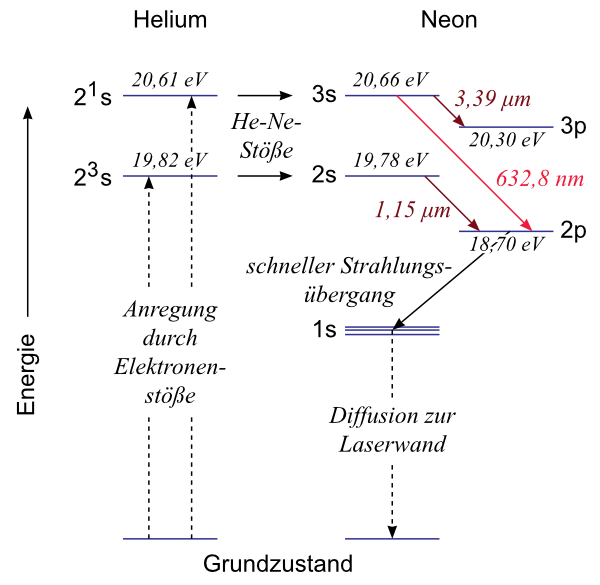
\includegraphics[scale=0.6]{NiveauHeNe.png}
	\caption{Niveauschema des Helium-Neon-Lasers. \cite[Datum: 02.01.15]{LP21}}
\end{figure}


\subsection{Beugung und Interferenz}

\subsubsection{Vom Kirchhoffschen Beugungsintegral zur Fraunhofer-Näherung}
Um das Feld eines bestrahlten Objektes in einer Ebene dahinter zu berechnen, integriert man über alle \emph{Elementarwellen} der Apertur:
\begin{align}
	E(x',y',z)=\frac{1}{i \lambda} \int \limits _{Apertur} E(x,y,0) ~ \frac{e^{ikr}}{r}~\dif x ~\dif y \quad \text{mit} ~ r^2=(x'-x)^2+(y'-y)^2+z^2 \,.
	\label{eq:Beugungsintegral}
\end{align}
Dies ist das \emph{Fresnel-Kirchhoffschen Beugungsintegral}.\\

Die \emph{Fresnel-Näherung} setzt voraus, dass die Bildebene weit entfernt von der Aperturebene ist, also $z \gg x'-x,~y'-y~$.
Dann vereinfacht sich der obige Ausdruck zu
\begin{align}
	E(x',y',z)=\frac{e^{ikz}}{i \lambda z} \int \limits _{Apertur} E(x,y,0) ~ \exp\left(\frac{ik}{2z}\left((x'-x)^2+(y'-y)^2\right)\right) ~\dif x ~\dif y\,.
	\label{eq:Fresnel}
\end{align}

Befindet man sich mit der Bildebene im \emph{Fernfeld}, kann man die \emph{Fraunhofer-Näherung} benutzen.
Dabei ist die Fresnel-Zahl $F=\frac{a^2}{\lambda z}$ mit der die Apertur charakterisierenden Größe $a$ sehr viel geringer als 1.
Also können die in x bzw. y quadratischen Terme vernachlässigt werden und man erhält

\begin{align}
	E(x',y',z)=\frac{e^{ikz} \cdot e^{i \frac{k_xx'+k_yy'}{2}}}{i \lambda z}\cdot \int \limits _{Apertur} E(x,y,0)~ e^{-ik_xx} ~ e^{-ik_yy} ~\dif x~ \dif y \,,
	\label{eq:Fraunhofer1}
\end{align}
mit $k_x:= k\frac{x'}{z}$ und  $k_y:= k\frac{y'}{z}$.\\

Das Fernfeld eines bestrahlten Objekts ergibt sich also als Fouriertransformation des Feldes in der Objektebene:
\begin{align}
	E(x',y',z)=B(x,y)\cdot \mathcal{F}\left[E(x,y,0)
	\right](k_x,k_y) \,.
	\label{eq:Fraunhofer2}
\end{align}

\subsubsection{Doppelspalt}
Für einen Doppelspalt mit einem Spaltabstand $d$ und infinitesimaler Spaltbreite ergibt sich nach \eqref{eq:Fraunhofer2} dieser Intensitätsverlauf
\begin{align}
	I(\varepsilon)=I_0 \cdot \cos^2(\varepsilon) \qquad \text{mit }\varepsilon= \frac{\pi d \sin \alpha}{\lambda}\,.
\end{align}
Man transformiert nämlich zwei Delta-Peaks.

\subsubsection{Einzelspalt und Steg}
Für einen Einzelspalt mit einer Spaltbreite $b$ ergibt sich nach \eqref{eq:Fraunhofer2} dieser Intensitätsverlauf
\begin{align}
	I(\varepsilon)=I_0 \cdot \sinc^2(\varepsilon)\qquad \text{mit }\varepsilon= \frac{\pi b \sin \alpha}{\lambda}\,.
\end{align}
Da das Fernfeld eines unendlichen Schirmes, also die Superposition aus Einzelspalt und Steg, perfekt dunkel ist, gilt:
$$ E_\text{Spalt} + E_\text{Steg} = 0 \,.$$
Da man nur die Intensität, also das Quadrat des E-Feldes, misst ergibt sich als Fernfeld des Stegs der Länge $b$ die gleiche Verteilung wie bei einem Einzelspalt gleicher Spaltbreite.

\subsubsection{Kreisblende}
Für eine Kreisblende mit dem Durchmesser $D$ ergibt sich -- nach etwas komplexerer Rechnung -- nach \eqref{eq:Fraunhofer2} dieser Intensitätsverlauf
\begin{align}
	I(\varepsilon)=I_0 \cdot \left(\frac{J_1(\varepsilon)}{\varepsilon}\right)^2 \qquad \text{mit }\varepsilon= \frac{\pi D \sin \alpha}{\lambda}\,.
\end{align}
Dabei ist $J_1$ die zylindrische Besselfunktion.
Das erste Minimum von $\left(\frac{J_1(\varepsilon)}{\varepsilon}\right)^2$ liegt bei 1.22.
Diese Zahl taucht auch beim Auflösungsvermögen bzw. Rayleigh-Kriterium auf.

\subsubsection{Mehrfachspalt}
Bei einem Mehrfachspalt, bei dem $N$ Spalte der Breite $b$ und dem Abstand $d$ beleuchtet werden, erhält man die Fernfeldverteilung aus dem Faltungssatz als Produkt aus Einzelpalteffekt und der Fouriertransformation von $N$ Delta-Peaks:
\begin{align}
	I(\varepsilon)=I_0 \cdot \sinc^2\left(\frac{\pi\alpha b}{\lambda}\right) \cdot \left(\frac{\sin(N\varepsilon)}{\sin(\varepsilon)}\right)^2 \qquad \text{mit }\varepsilon= \frac{\pi d \sin \alpha}{\lambda}\,.
\end{align}

\section{Durchführung}
\label{sec:durchfuehrung}
\begin{figure}[!h]
	\centering
	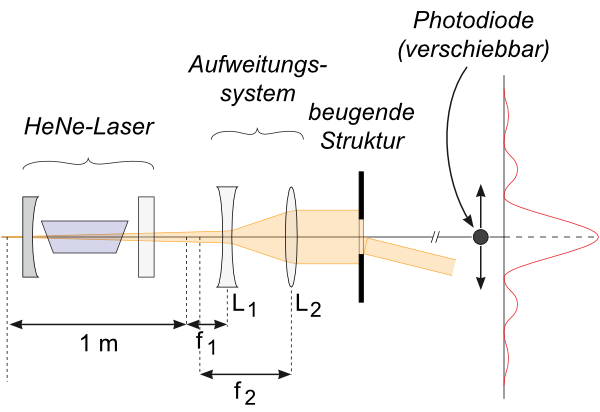
\includegraphics[scale=0.7]{Aufbau.png}
	\caption{Aufbau. \cite[Datum: 02.01.15]{LP21}}
\end{figure}

Um die Messergebnisse nicht zu verfälschen ist es immens wichtig, die Beugungsobjekte nur an der Fassung anzufassen.
Genauso vorsichtig soll auch mit den Linsen umgegangen werden.\\

Zuerst schaltet man den PC an und meldet sich unter dem Benutzer ''laser'' ohne Passwort an.
Dann startet man das Programm \emph{Lasersteuerung} auf dem Desktop.
Der Motor der Fotodiode bewegt sich dann auf die Nullposition.
Nun kann der Laser mittels Schiebeschalter auf der Rückseite angeschaltet werden.\\

Vor jeder Messung weitet man das Strahlenbündel mit Zerstreungs- und Sammellinse auf, sodass das gesamte Objekt homogen, parallel und ausreichend breit beleuchtet wird.
Außerdem überlegt man sich, welche Beugungsmuster zu erwarten sind.\\

Nun beginnt die Messung.
Um eine möglichst parallele Bestrahlung zu ermöglichen, muss der Abstand zwischen Objekt und Laserdiode möglichst groß sein.
Außerdem soll er gemessen werden.
Zuerst stellt man im Programm ein, von wo bis wo die Diode den Verlauf aufnehmen soll ($400~$Schritte $\corresponds 1~$mm) und welcher Spannungsbereich erfasst werden soll.
Dabei kann man je nach Intensität zwischen $0-1~$V und $0-10~$V wählen.

Die symmetrischen Spektren sollen bis zum vierten Nebenmaximum -- links wie rechts -- vom Hauptmaximum aufgenommen werden.
Außerdem genügt es beim Gitter sowie bei der Doppellochblende, nur bis zum ersten Nebenmaximum des Einzelspalteffektes bzw. der Blendenfunktion zu messen, da die Intensität danach zu gering ist.
Außerdem sollen alle Extrema deutlich bestimmt werden.
Dazu ist es wichtig den richtigen Messbereich auszuwählen, da am Rand die Maxima sehr schwach sind.
Also werden zwei Messungen durchgeführt: einmal das Zentrum und danach die Randgebiete.
In welchem Messbereich man sich befindet, kann man an der Anzeige der aktuellen Fotospannung ablesen.\\

Die Fotodiode wird mit der  manuellen Steuerung im oberen Teil des Programmfensters zuerst an die beiden Ränder der bevorstehenden Messung gefahren, die Positionswerte werden notiert und dann als Grenzen der Messung eingeben.
Nun muss noch die Schrittweite eingegeben werden.
Sie sollte unter 50 Schritten, also einem Achtel Millimeter liegen.
Im Fenster unten links wird dann der automatische Messvorgang gestartet.
Das Spektrum wird abgespeichert und mit einem Plotprogramm dargestellt, beschriftet und schließlich ausgedruckt.
Dies dient als Messprotokoll.
Neben dem Beugungsobjekt und den Achsen mit Einheiten sollen noch der Konversionsfaktor in Schritten/mm, der Objektabstand von der Diode sowie die Wellenlänge des Lasers als auch die charakteristische Größe des Objekts enthalten.\\

Schließlich werden alle Daten auf einem USB-Stick gespeichert.

\section{Auswertung}
\label{sec:auswertung}
\subsection{Objektgrößen bestimmen}
\begin{align}
	D&=\frac{\frac{\varepsilon}{\pi}}{\alpha}\lambda=\frac{\lambda}{m}\,,\\
	\sigma_D&=\frac{\lambda}{m^2}\cdot \sigma_m\,.
\end{align}

\begin{figure}[!htb]
	\centering
	% GNUPLOT: LaTeX picture with Postscript
\begingroup
  \makeatletter
  \providecommand\color[2][]{%
    \GenericError{(gnuplot) \space\space\space\@spaces}{%
      Package color not loaded in conjunction with
      terminal option `colourtext'%
    }{See the gnuplot documentation for explanation.%
    }{Either use 'blacktext' in gnuplot or load the package
      color.sty in LaTeX.}%
    \renewcommand\color[2][]{}%
  }%
  \providecommand\includegraphics[2][]{%
    \GenericError{(gnuplot) \space\space\space\@spaces}{%
      Package graphicx or graphics not loaded%
    }{See the gnuplot documentation for explanation.%
    }{The gnuplot epslatex terminal needs graphicx.sty or graphics.sty.}%
    \renewcommand\includegraphics[2][]{}%
  }%
  \providecommand\rotatebox[2]{#2}%
  \@ifundefined{ifGPcolor}{%
    \newif\ifGPcolor
    \GPcolortrue
  }{}%
  \@ifundefined{ifGPblacktext}{%
    \newif\ifGPblacktext
    \GPblacktexttrue
  }{}%
  % define a \g@addto@macro without @ in the name:
  \let\gplgaddtomacro\g@addto@macro
  % define empty templates for all commands taking text:
  \gdef\gplbacktext{}%
  \gdef\gplfronttext{}%
  \makeatother
  \ifGPblacktext
    % no textcolor at all
    \def\colorrgb#1{}%
    \def\colorgray#1{}%
  \else
    % gray or color?
    \ifGPcolor
      \def\colorrgb#1{\color[rgb]{#1}}%
      \def\colorgray#1{\color[gray]{#1}}%
      \expandafter\def\csname LTw\endcsname{\color{white}}%
      \expandafter\def\csname LTb\endcsname{\color{black}}%
      \expandafter\def\csname LTa\endcsname{\color{black}}%
      \expandafter\def\csname LT0\endcsname{\color[rgb]{1,0,0}}%
      \expandafter\def\csname LT1\endcsname{\color[rgb]{0,1,0}}%
      \expandafter\def\csname LT2\endcsname{\color[rgb]{0,0,1}}%
      \expandafter\def\csname LT3\endcsname{\color[rgb]{1,0,1}}%
      \expandafter\def\csname LT4\endcsname{\color[rgb]{0,1,1}}%
      \expandafter\def\csname LT5\endcsname{\color[rgb]{1,1,0}}%
      \expandafter\def\csname LT6\endcsname{\color[rgb]{0,0,0}}%
      \expandafter\def\csname LT7\endcsname{\color[rgb]{1,0.3,0}}%
      \expandafter\def\csname LT8\endcsname{\color[rgb]{0.5,0.5,0.5}}%
    \else
      % gray
      \def\colorrgb#1{\color{black}}%
      \def\colorgray#1{\color[gray]{#1}}%
      \expandafter\def\csname LTw\endcsname{\color{white}}%
      \expandafter\def\csname LTb\endcsname{\color{black}}%
      \expandafter\def\csname LTa\endcsname{\color{black}}%
      \expandafter\def\csname LT0\endcsname{\color{black}}%
      \expandafter\def\csname LT1\endcsname{\color{black}}%
      \expandafter\def\csname LT2\endcsname{\color{black}}%
      \expandafter\def\csname LT3\endcsname{\color{black}}%
      \expandafter\def\csname LT4\endcsname{\color{black}}%
      \expandafter\def\csname LT5\endcsname{\color{black}}%
      \expandafter\def\csname LT6\endcsname{\color{black}}%
      \expandafter\def\csname LT7\endcsname{\color{black}}%
      \expandafter\def\csname LT8\endcsname{\color{black}}%
    \fi
  \fi
  \setlength{\unitlength}{0.0500bp}%
  \begin{picture}(7200.00,5040.00)%
    \gplgaddtomacro\gplbacktext{%
      \csname LTb\endcsname%
      \put(1518,704){\makebox(0,0)[r]{\strut{}-0.015}}%
      \put(1518,1383){\makebox(0,0)[r]{\strut{}-0.01}}%
      \put(1518,2061){\makebox(0,0)[r]{\strut{}-0.005}}%
      \put(1518,2740){\makebox(0,0)[r]{\strut{} 0}}%
      \put(1518,3419){\makebox(0,0)[r]{\strut{} 0.005}}%
      \put(1518,4097){\makebox(0,0)[r]{\strut{} 0.01}}%
      \put(1518,4776){\makebox(0,0)[r]{\strut{} 0.015}}%
      \put(1650,484){\makebox(0,0){\strut{}-4}}%
      \put(2314,484){\makebox(0,0){\strut{}-3}}%
      \put(2977,484){\makebox(0,0){\strut{}-2}}%
      \put(3641,484){\makebox(0,0){\strut{}-1}}%
      \put(4304,484){\makebox(0,0){\strut{} 0}}%
      \put(4968,484){\makebox(0,0){\strut{} 1}}%
      \put(5631,484){\makebox(0,0){\strut{} 2}}%
      \put(6295,484){\makebox(0,0){\strut{} 3}}%
      \put(6958,484){\makebox(0,0){\strut{} 4}}%
      \put(484,2740){\rotatebox{90}{\makebox(0,0){\strut{}$\alpha_i$}}}%
      \put(4304,154){\makebox(0,0){\strut{}$\frac{\varepsilon_i}{\pi}$}}%
      \put(2314,4097){\makebox(0,0)[l]{\strut{}$m = (2930 \pm  10)~10^{-6} $}}%
      \put(2314,3690){\makebox(0,0)[l]{\strut{}$b = (-56 \pm  26)~10^{-6} $}}%
    }%
    \gplgaddtomacro\gplfronttext{%
      \csname LTb\endcsname%
      \put(5971,1097){\makebox(0,0)[r]{\strut{}Extrema}}%
      \csname LTb\endcsname%
      \put(5971,877){\makebox(0,0)[r]{\strut{}$\alpha=m \cdot \frac{\varepsilon}{\pi}+b $}}%
    }%
    \gplbacktext
    \put(0,0){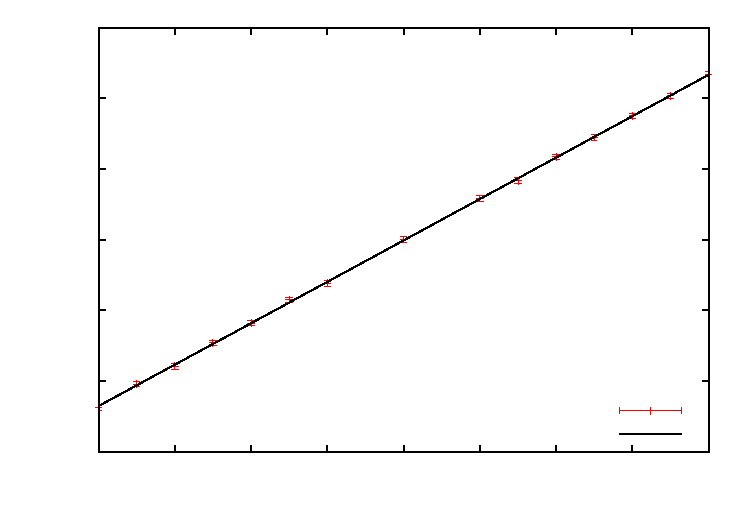
\includegraphics{spalt_reg}}%
    \gplfronttext
  \end{picture}%
\endgroup

	\caption{Spalt}
\end{figure}

\begin{figure}[!htb]
	\centering
	% GNUPLOT: LaTeX picture with Postscript
\begingroup
  \makeatletter
  \providecommand\color[2][]{%
    \GenericError{(gnuplot) \space\space\space\@spaces}{%
      Package color not loaded in conjunction with
      terminal option `colourtext'%
    }{See the gnuplot documentation for explanation.%
    }{Either use 'blacktext' in gnuplot or load the package
      color.sty in LaTeX.}%
    \renewcommand\color[2][]{}%
  }%
  \providecommand\includegraphics[2][]{%
    \GenericError{(gnuplot) \space\space\space\@spaces}{%
      Package graphicx or graphics not loaded%
    }{See the gnuplot documentation for explanation.%
    }{The gnuplot epslatex terminal needs graphicx.sty or graphics.sty.}%
    \renewcommand\includegraphics[2][]{}%
  }%
  \providecommand\rotatebox[2]{#2}%
  \@ifundefined{ifGPcolor}{%
    \newif\ifGPcolor
    \GPcolortrue
  }{}%
  \@ifundefined{ifGPblacktext}{%
    \newif\ifGPblacktext
    \GPblacktexttrue
  }{}%
  % define a \g@addto@macro without @ in the name:
  \let\gplgaddtomacro\g@addto@macro
  % define empty templates for all commands taking text:
  \gdef\gplbacktext{}%
  \gdef\gplfronttext{}%
  \makeatother
  \ifGPblacktext
    % no textcolor at all
    \def\colorrgb#1{}%
    \def\colorgray#1{}%
  \else
    % gray or color?
    \ifGPcolor
      \def\colorrgb#1{\color[rgb]{#1}}%
      \def\colorgray#1{\color[gray]{#1}}%
      \expandafter\def\csname LTw\endcsname{\color{white}}%
      \expandafter\def\csname LTb\endcsname{\color{black}}%
      \expandafter\def\csname LTa\endcsname{\color{black}}%
      \expandafter\def\csname LT0\endcsname{\color[rgb]{1,0,0}}%
      \expandafter\def\csname LT1\endcsname{\color[rgb]{0,1,0}}%
      \expandafter\def\csname LT2\endcsname{\color[rgb]{0,0,1}}%
      \expandafter\def\csname LT3\endcsname{\color[rgb]{1,0,1}}%
      \expandafter\def\csname LT4\endcsname{\color[rgb]{0,1,1}}%
      \expandafter\def\csname LT5\endcsname{\color[rgb]{1,1,0}}%
      \expandafter\def\csname LT6\endcsname{\color[rgb]{0,0,0}}%
      \expandafter\def\csname LT7\endcsname{\color[rgb]{1,0.3,0}}%
      \expandafter\def\csname LT8\endcsname{\color[rgb]{0.5,0.5,0.5}}%
    \else
      % gray
      \def\colorrgb#1{\color{black}}%
      \def\colorgray#1{\color[gray]{#1}}%
      \expandafter\def\csname LTw\endcsname{\color{white}}%
      \expandafter\def\csname LTb\endcsname{\color{black}}%
      \expandafter\def\csname LTa\endcsname{\color{black}}%
      \expandafter\def\csname LT0\endcsname{\color{black}}%
      \expandafter\def\csname LT1\endcsname{\color{black}}%
      \expandafter\def\csname LT2\endcsname{\color{black}}%
      \expandafter\def\csname LT3\endcsname{\color{black}}%
      \expandafter\def\csname LT4\endcsname{\color{black}}%
      \expandafter\def\csname LT5\endcsname{\color{black}}%
      \expandafter\def\csname LT6\endcsname{\color{black}}%
      \expandafter\def\csname LT7\endcsname{\color{black}}%
      \expandafter\def\csname LT8\endcsname{\color{black}}%
    \fi
  \fi
  \setlength{\unitlength}{0.0500bp}%
  \begin{picture}(7200.00,5040.00)%
    \gplgaddtomacro\gplbacktext{%
      \csname LTb\endcsname%
      \put(1518,704){\makebox(0,0)[r]{\strut{}-0.015}}%
      \put(1518,1383){\makebox(0,0)[r]{\strut{}-0.01}}%
      \put(1518,2061){\makebox(0,0)[r]{\strut{}-0.005}}%
      \put(1518,2740){\makebox(0,0)[r]{\strut{} 0}}%
      \put(1518,3419){\makebox(0,0)[r]{\strut{} 0.005}}%
      \put(1518,4097){\makebox(0,0)[r]{\strut{} 0.01}}%
      \put(1518,4776){\makebox(0,0)[r]{\strut{} 0.015}}%
      \put(1650,484){\makebox(0,0){\strut{}-4}}%
      \put(2314,484){\makebox(0,0){\strut{}-3}}%
      \put(2977,484){\makebox(0,0){\strut{}-2}}%
      \put(3641,484){\makebox(0,0){\strut{}-1}}%
      \put(4304,484){\makebox(0,0){\strut{} 0}}%
      \put(4968,484){\makebox(0,0){\strut{} 1}}%
      \put(5631,484){\makebox(0,0){\strut{} 2}}%
      \put(6295,484){\makebox(0,0){\strut{} 3}}%
      \put(6958,484){\makebox(0,0){\strut{} 4}}%
      \put(484,2740){\rotatebox{90}{\makebox(0,0){\strut{}$\alpha_i$}}}%
      \put(4304,154){\makebox(0,0){\strut{}$\frac{\varepsilon_i}{\pi}$}}%
      \put(2314,4097){\makebox(0,0)[l]{\strut{}$m = (3292 \pm  10)~10^{-6} $}}%
      \put(2314,3690){\makebox(0,0)[l]{\strut{}$b = ( 24 \pm  26)~10^{-6} $}}%
    }%
    \gplgaddtomacro\gplfronttext{%
      \csname LTb\endcsname%
      \put(5971,1097){\makebox(0,0)[r]{\strut{}Extrema}}%
      \csname LTb\endcsname%
      \put(5971,877){\makebox(0,0)[r]{\strut{}$\alpha=m \cdot \frac{\varepsilon}{\pi}+b $}}%
    }%
    \gplbacktext
    \put(0,0){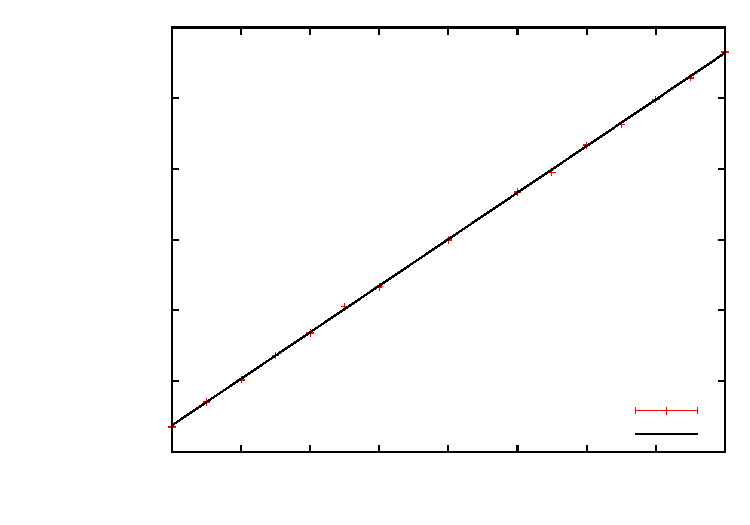
\includegraphics{steg_reg}}%
    \gplfronttext
  \end{picture}%
\endgroup

	\caption{Steg}
\end{figure}

\begin{figure}[!htb]
	\centering
	% GNUPLOT: LaTeX picture with Postscript
\begingroup
  \makeatletter
  \providecommand\color[2][]{%
    \GenericError{(gnuplot) \space\space\space\@spaces}{%
      Package color not loaded in conjunction with
      terminal option `colourtext'%
    }{See the gnuplot documentation for explanation.%
    }{Either use 'blacktext' in gnuplot or load the package
      color.sty in LaTeX.}%
    \renewcommand\color[2][]{}%
  }%
  \providecommand\includegraphics[2][]{%
    \GenericError{(gnuplot) \space\space\space\@spaces}{%
      Package graphicx or graphics not loaded%
    }{See the gnuplot documentation for explanation.%
    }{The gnuplot epslatex terminal needs graphicx.sty or graphics.sty.}%
    \renewcommand\includegraphics[2][]{}%
  }%
  \providecommand\rotatebox[2]{#2}%
  \@ifundefined{ifGPcolor}{%
    \newif\ifGPcolor
    \GPcolortrue
  }{}%
  \@ifundefined{ifGPblacktext}{%
    \newif\ifGPblacktext
    \GPblacktexttrue
  }{}%
  % define a \g@addto@macro without @ in the name:
  \let\gplgaddtomacro\g@addto@macro
  % define empty templates for all commands taking text:
  \gdef\gplbacktext{}%
  \gdef\gplfronttext{}%
  \makeatother
  \ifGPblacktext
    % no textcolor at all
    \def\colorrgb#1{}%
    \def\colorgray#1{}%
  \else
    % gray or color?
    \ifGPcolor
      \def\colorrgb#1{\color[rgb]{#1}}%
      \def\colorgray#1{\color[gray]{#1}}%
      \expandafter\def\csname LTw\endcsname{\color{white}}%
      \expandafter\def\csname LTb\endcsname{\color{black}}%
      \expandafter\def\csname LTa\endcsname{\color{black}}%
      \expandafter\def\csname LT0\endcsname{\color[rgb]{1,0,0}}%
      \expandafter\def\csname LT1\endcsname{\color[rgb]{0,1,0}}%
      \expandafter\def\csname LT2\endcsname{\color[rgb]{0,0,1}}%
      \expandafter\def\csname LT3\endcsname{\color[rgb]{1,0,1}}%
      \expandafter\def\csname LT4\endcsname{\color[rgb]{0,1,1}}%
      \expandafter\def\csname LT5\endcsname{\color[rgb]{1,1,0}}%
      \expandafter\def\csname LT6\endcsname{\color[rgb]{0,0,0}}%
      \expandafter\def\csname LT7\endcsname{\color[rgb]{1,0.3,0}}%
      \expandafter\def\csname LT8\endcsname{\color[rgb]{0.5,0.5,0.5}}%
    \else
      % gray
      \def\colorrgb#1{\color{black}}%
      \def\colorgray#1{\color[gray]{#1}}%
      \expandafter\def\csname LTw\endcsname{\color{white}}%
      \expandafter\def\csname LTb\endcsname{\color{black}}%
      \expandafter\def\csname LTa\endcsname{\color{black}}%
      \expandafter\def\csname LT0\endcsname{\color{black}}%
      \expandafter\def\csname LT1\endcsname{\color{black}}%
      \expandafter\def\csname LT2\endcsname{\color{black}}%
      \expandafter\def\csname LT3\endcsname{\color{black}}%
      \expandafter\def\csname LT4\endcsname{\color{black}}%
      \expandafter\def\csname LT5\endcsname{\color{black}}%
      \expandafter\def\csname LT6\endcsname{\color{black}}%
      \expandafter\def\csname LT7\endcsname{\color{black}}%
      \expandafter\def\csname LT8\endcsname{\color{black}}%
    \fi
  \fi
  \setlength{\unitlength}{0.0500bp}%
  \begin{picture}(7200.00,5040.00)%
    \gplgaddtomacro\gplbacktext{%
      \csname LTb\endcsname%
      \put(1518,704){\makebox(0,0)[r]{\strut{}-0.015}}%
      \put(1518,1383){\makebox(0,0)[r]{\strut{}-0.01}}%
      \put(1518,2061){\makebox(0,0)[r]{\strut{}-0.005}}%
      \put(1518,2740){\makebox(0,0)[r]{\strut{} 0}}%
      \put(1518,3419){\makebox(0,0)[r]{\strut{} 0.005}}%
      \put(1518,4097){\makebox(0,0)[r]{\strut{} 0.01}}%
      \put(1518,4776){\makebox(0,0)[r]{\strut{} 0.015}}%
      \put(1650,484){\makebox(0,0){\strut{}-4}}%
      \put(2240,484){\makebox(0,0){\strut{}-3}}%
      \put(2830,484){\makebox(0,0){\strut{}-2}}%
      \put(3419,484){\makebox(0,0){\strut{}-1}}%
      \put(4009,484){\makebox(0,0){\strut{} 0}}%
      \put(4599,484){\makebox(0,0){\strut{} 1}}%
      \put(5189,484){\makebox(0,0){\strut{} 2}}%
      \put(5778,484){\makebox(0,0){\strut{} 3}}%
      \put(6368,484){\makebox(0,0){\strut{} 4}}%
      \put(6958,484){\makebox(0,0){\strut{} 5}}%
      \put(484,2740){\rotatebox{90}{\makebox(0,0){\strut{}$\alpha_i$}}}%
      \put(4304,154){\makebox(0,0){\strut{}$\frac{\varepsilon_i}{\pi}$}}%
      \put(2240,4097){\makebox(0,0)[l]{\strut{}$m = (3312 \pm   7)~10^{-6} $}}%
      \put(2240,3690){\makebox(0,0)[l]{\strut{}$b = (-18 \pm  18)~10^{-6} $}}%
    }%
    \gplgaddtomacro\gplfronttext{%
      \csname LTb\endcsname%
      \put(5971,1097){\makebox(0,0)[r]{\strut{}Extrema}}%
      \csname LTb\endcsname%
      \put(5971,877){\makebox(0,0)[r]{\strut{}$\alpha=m \cdot \frac{\varepsilon}{\pi}+b $}}%
    }%
    \gplbacktext
    \put(0,0){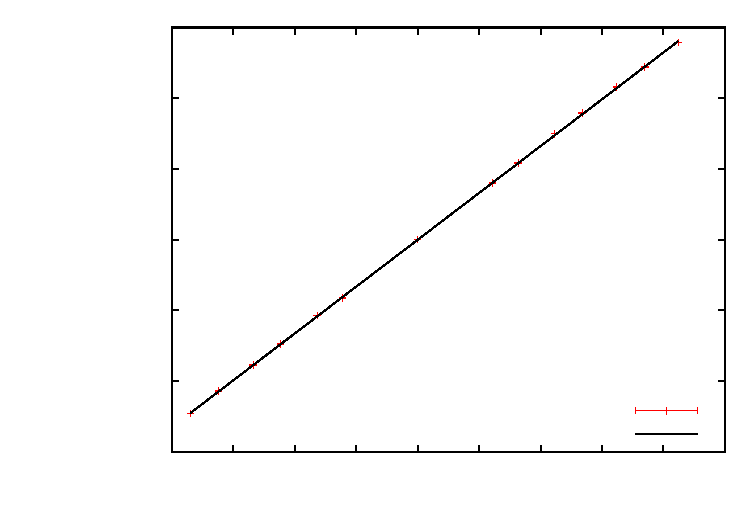
\includegraphics{loch_reg}}%
    \gplfronttext
  \end{picture}%
\endgroup

	\caption{Lochblende}
\end{figure}

\begin{figure}[!htb]
	\centering
	% GNUPLOT: LaTeX picture with Postscript
\begingroup
  \makeatletter
  \providecommand\color[2][]{%
    \GenericError{(gnuplot) \space\space\space\@spaces}{%
      Package color not loaded in conjunction with
      terminal option `colourtext'%
    }{See the gnuplot documentation for explanation.%
    }{Either use 'blacktext' in gnuplot or load the package
      color.sty in LaTeX.}%
    \renewcommand\color[2][]{}%
  }%
  \providecommand\includegraphics[2][]{%
    \GenericError{(gnuplot) \space\space\space\@spaces}{%
      Package graphicx or graphics not loaded%
    }{See the gnuplot documentation for explanation.%
    }{The gnuplot epslatex terminal needs graphicx.sty or graphics.sty.}%
    \renewcommand\includegraphics[2][]{}%
  }%
  \providecommand\rotatebox[2]{#2}%
  \@ifundefined{ifGPcolor}{%
    \newif\ifGPcolor
    \GPcolortrue
  }{}%
  \@ifundefined{ifGPblacktext}{%
    \newif\ifGPblacktext
    \GPblacktexttrue
  }{}%
  % define a \g@addto@macro without @ in the name:
  \let\gplgaddtomacro\g@addto@macro
  % define empty templates for all commands taking text:
  \gdef\gplbacktext{}%
  \gdef\gplfronttext{}%
  \makeatother
  \ifGPblacktext
    % no textcolor at all
    \def\colorrgb#1{}%
    \def\colorgray#1{}%
  \else
    % gray or color?
    \ifGPcolor
      \def\colorrgb#1{\color[rgb]{#1}}%
      \def\colorgray#1{\color[gray]{#1}}%
      \expandafter\def\csname LTw\endcsname{\color{white}}%
      \expandafter\def\csname LTb\endcsname{\color{black}}%
      \expandafter\def\csname LTa\endcsname{\color{black}}%
      \expandafter\def\csname LT0\endcsname{\color[rgb]{1,0,0}}%
      \expandafter\def\csname LT1\endcsname{\color[rgb]{0,1,0}}%
      \expandafter\def\csname LT2\endcsname{\color[rgb]{0,0,1}}%
      \expandafter\def\csname LT3\endcsname{\color[rgb]{1,0,1}}%
      \expandafter\def\csname LT4\endcsname{\color[rgb]{0,1,1}}%
      \expandafter\def\csname LT5\endcsname{\color[rgb]{1,1,0}}%
      \expandafter\def\csname LT6\endcsname{\color[rgb]{0,0,0}}%
      \expandafter\def\csname LT7\endcsname{\color[rgb]{1,0.3,0}}%
      \expandafter\def\csname LT8\endcsname{\color[rgb]{0.5,0.5,0.5}}%
    \else
      % gray
      \def\colorrgb#1{\color{black}}%
      \def\colorgray#1{\color[gray]{#1}}%
      \expandafter\def\csname LTw\endcsname{\color{white}}%
      \expandafter\def\csname LTb\endcsname{\color{black}}%
      \expandafter\def\csname LTa\endcsname{\color{black}}%
      \expandafter\def\csname LT0\endcsname{\color{black}}%
      \expandafter\def\csname LT1\endcsname{\color{black}}%
      \expandafter\def\csname LT2\endcsname{\color{black}}%
      \expandafter\def\csname LT3\endcsname{\color{black}}%
      \expandafter\def\csname LT4\endcsname{\color{black}}%
      \expandafter\def\csname LT5\endcsname{\color{black}}%
      \expandafter\def\csname LT6\endcsname{\color{black}}%
      \expandafter\def\csname LT7\endcsname{\color{black}}%
      \expandafter\def\csname LT8\endcsname{\color{black}}%
    \fi
  \fi
  \setlength{\unitlength}{0.0500bp}%
  \begin{picture}(7200.00,5040.00)%
    \gplgaddtomacro\gplbacktext{%
      \csname LTb\endcsname%
      \put(682,704){\makebox(0,0)[r]{\strut{}-3}}%
      \put(682,1383){\makebox(0,0)[r]{\strut{}-2}}%
      \put(682,2061){\makebox(0,0)[r]{\strut{}-1}}%
      \put(682,2740){\makebox(0,0)[r]{\strut{} 0}}%
      \put(682,3418){\makebox(0,0)[r]{\strut{} 1}}%
      \put(682,4097){\makebox(0,0)[r]{\strut{} 2}}%
      \put(682,4775){\makebox(0,0)[r]{\strut{} 3}}%
      \put(814,484){\makebox(0,0){\strut{}-2}}%
      \put(1563,484){\makebox(0,0){\strut{}-1.5}}%
      \put(2311,484){\makebox(0,0){\strut{}-1}}%
      \put(3060,484){\makebox(0,0){\strut{}-0.5}}%
      \put(3809,484){\makebox(0,0){\strut{} 0}}%
      \put(4557,484){\makebox(0,0){\strut{} 0.5}}%
      \put(5306,484){\makebox(0,0){\strut{} 1}}%
      \put(6054,484){\makebox(0,0){\strut{} 1.5}}%
      \put(6803,484){\makebox(0,0){\strut{} 2}}%
      \put(176,2739){\rotatebox{-270}{\makebox(0,0){\strut{}$\alpha_i$ [$10^{-3}~$rad]}}}%
      \put(3808,154){\makebox(0,0){\strut{}$\frac{\varepsilon_i}{\pi}$ [rad]}}%
      \put(1563,4097){\makebox(0,0)[l]{\strut{}$m = (1.3027 \pm 0.0195)~10^{-3}$}}%
      \put(1563,3689){\makebox(0,0)[l]{\strut{}$b = (0.0102 \pm 0.0251)~10^{-3}$}}%
      \put(1563,3282){\makebox(0,0)[l]{\strut{}$r = 0.99922 $}}%
    }%
    \gplgaddtomacro\gplfronttext{%
      \csname LTb\endcsname%
      \put(5816,1097){\makebox(0,0)[r]{\strut{}Extrema}}%
      \csname LTb\endcsname%
      \put(5816,877){\makebox(0,0)[r]{\strut{}$\alpha=m \cdot \frac{\varepsilon}{\pi}+b $}}%
    }%
    \gplbacktext
    \put(0,0){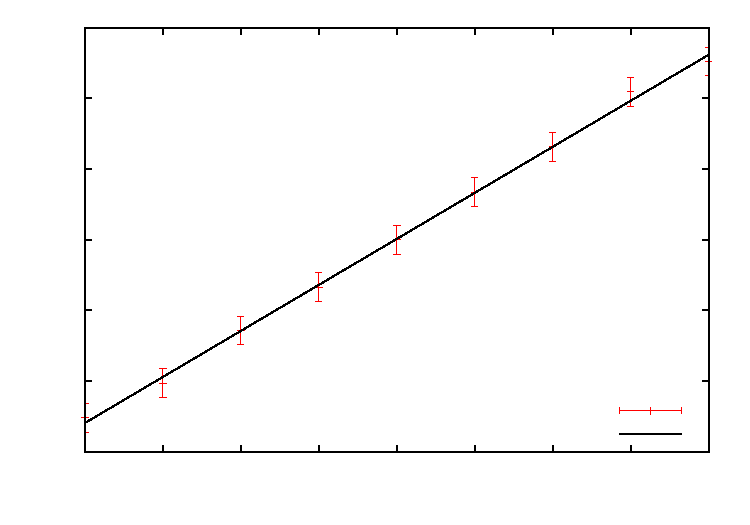
\includegraphics{doppelloch1_reg}}%
    \gplfronttext
  \end{picture}%
\endgroup

	\caption{Doppelloch-Blende mit kleinstem Lochabstand}
\end{figure}

\begin{figure}[!htb]
	\centering
	% GNUPLOT: LaTeX picture with Postscript
\begingroup
  \makeatletter
  \providecommand\color[2][]{%
    \GenericError{(gnuplot) \space\space\space\@spaces}{%
      Package color not loaded in conjunction with
      terminal option `colourtext'%
    }{See the gnuplot documentation for explanation.%
    }{Either use 'blacktext' in gnuplot or load the package
      color.sty in LaTeX.}%
    \renewcommand\color[2][]{}%
  }%
  \providecommand\includegraphics[2][]{%
    \GenericError{(gnuplot) \space\space\space\@spaces}{%
      Package graphicx or graphics not loaded%
    }{See the gnuplot documentation for explanation.%
    }{The gnuplot epslatex terminal needs graphicx.sty or graphics.sty.}%
    \renewcommand\includegraphics[2][]{}%
  }%
  \providecommand\rotatebox[2]{#2}%
  \@ifundefined{ifGPcolor}{%
    \newif\ifGPcolor
    \GPcolortrue
  }{}%
  \@ifundefined{ifGPblacktext}{%
    \newif\ifGPblacktext
    \GPblacktexttrue
  }{}%
  % define a \g@addto@macro without @ in the name:
  \let\gplgaddtomacro\g@addto@macro
  % define empty templates for all commands taking text:
  \gdef\gplbacktext{}%
  \gdef\gplfronttext{}%
  \makeatother
  \ifGPblacktext
    % no textcolor at all
    \def\colorrgb#1{}%
    \def\colorgray#1{}%
  \else
    % gray or color?
    \ifGPcolor
      \def\colorrgb#1{\color[rgb]{#1}}%
      \def\colorgray#1{\color[gray]{#1}}%
      \expandafter\def\csname LTw\endcsname{\color{white}}%
      \expandafter\def\csname LTb\endcsname{\color{black}}%
      \expandafter\def\csname LTa\endcsname{\color{black}}%
      \expandafter\def\csname LT0\endcsname{\color[rgb]{1,0,0}}%
      \expandafter\def\csname LT1\endcsname{\color[rgb]{0,1,0}}%
      \expandafter\def\csname LT2\endcsname{\color[rgb]{0,0,1}}%
      \expandafter\def\csname LT3\endcsname{\color[rgb]{1,0,1}}%
      \expandafter\def\csname LT4\endcsname{\color[rgb]{0,1,1}}%
      \expandafter\def\csname LT5\endcsname{\color[rgb]{1,1,0}}%
      \expandafter\def\csname LT6\endcsname{\color[rgb]{0,0,0}}%
      \expandafter\def\csname LT7\endcsname{\color[rgb]{1,0.3,0}}%
      \expandafter\def\csname LT8\endcsname{\color[rgb]{0.5,0.5,0.5}}%
    \else
      % gray
      \def\colorrgb#1{\color{black}}%
      \def\colorgray#1{\color[gray]{#1}}%
      \expandafter\def\csname LTw\endcsname{\color{white}}%
      \expandafter\def\csname LTb\endcsname{\color{black}}%
      \expandafter\def\csname LTa\endcsname{\color{black}}%
      \expandafter\def\csname LT0\endcsname{\color{black}}%
      \expandafter\def\csname LT1\endcsname{\color{black}}%
      \expandafter\def\csname LT2\endcsname{\color{black}}%
      \expandafter\def\csname LT3\endcsname{\color{black}}%
      \expandafter\def\csname LT4\endcsname{\color{black}}%
      \expandafter\def\csname LT5\endcsname{\color{black}}%
      \expandafter\def\csname LT6\endcsname{\color{black}}%
      \expandafter\def\csname LT7\endcsname{\color{black}}%
      \expandafter\def\csname LT8\endcsname{\color{black}}%
    \fi
  \fi
  \setlength{\unitlength}{0.0500bp}%
  \begin{picture}(7200.00,5040.00)%
    \gplgaddtomacro\gplbacktext{%
      \csname LTb\endcsname%
      \put(1650,704){\makebox(0,0)[r]{\strut{}-0.002}}%
      \put(1650,1111){\makebox(0,0)[r]{\strut{}-0.0015}}%
      \put(1650,1518){\makebox(0,0)[r]{\strut{}-0.001}}%
      \put(1650,1926){\makebox(0,0)[r]{\strut{}-0.0005}}%
      \put(1650,2333){\makebox(0,0)[r]{\strut{} 0}}%
      \put(1650,2740){\makebox(0,0)[r]{\strut{} 0.0005}}%
      \put(1650,3147){\makebox(0,0)[r]{\strut{} 0.001}}%
      \put(1650,3554){\makebox(0,0)[r]{\strut{} 0.0015}}%
      \put(1650,3962){\makebox(0,0)[r]{\strut{} 0.002}}%
      \put(1650,4369){\makebox(0,0)[r]{\strut{} 0.0025}}%
      \put(1650,4776){\makebox(0,0)[r]{\strut{} 0.003}}%
      \put(1782,484){\makebox(0,0){\strut{}-3}}%
      \put(2521,484){\makebox(0,0){\strut{}-2}}%
      \put(3261,484){\makebox(0,0){\strut{}-1}}%
      \put(4000,484){\makebox(0,0){\strut{} 0}}%
      \put(4740,484){\makebox(0,0){\strut{} 1}}%
      \put(5479,484){\makebox(0,0){\strut{} 2}}%
      \put(6219,484){\makebox(0,0){\strut{} 3}}%
      \put(6958,484){\makebox(0,0){\strut{} 4}}%
      \put(484,2740){\rotatebox{90}{\makebox(0,0){\strut{}$\alpha_i$}}}%
      \put(4370,154){\makebox(0,0){\strut{}$\frac{\varepsilon_i}{\pi}$}}%
      \put(2521,3962){\makebox(0,0)[l]{\strut{}$m = (681 \pm   8)~10^{-6} $}}%
      \put(2521,3554){\makebox(0,0)[l]{\strut{}$b = ( 71 \pm  17)~10^{-6} $}}%
    }%
    \gplgaddtomacro\gplfronttext{%
      \csname LTb\endcsname%
      \put(5971,1097){\makebox(0,0)[r]{\strut{}Extrema}}%
      \csname LTb\endcsname%
      \put(5971,877){\makebox(0,0)[r]{\strut{}$\alpha=m \cdot \frac{\varepsilon}{\pi}+b $}}%
    }%
    \gplbacktext
    \put(0,0){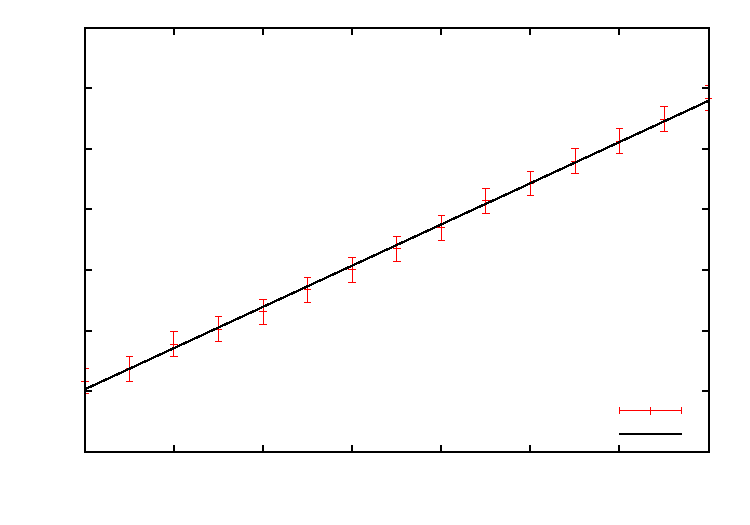
\includegraphics{doppelloch2_reg}}%
    \gplfronttext
  \end{picture}%
\endgroup

	\caption{Doppelloch-Blende mit mittlerem Lochabstand}
\end{figure}

\begin{figure}[!htb]
	\centering
	% GNUPLOT: LaTeX picture with Postscript
\begingroup
  \makeatletter
  \providecommand\color[2][]{%
    \GenericError{(gnuplot) \space\space\space\@spaces}{%
      Package color not loaded in conjunction with
      terminal option `colourtext'%
    }{See the gnuplot documentation for explanation.%
    }{Either use 'blacktext' in gnuplot or load the package
      color.sty in LaTeX.}%
    \renewcommand\color[2][]{}%
  }%
  \providecommand\includegraphics[2][]{%
    \GenericError{(gnuplot) \space\space\space\@spaces}{%
      Package graphicx or graphics not loaded%
    }{See the gnuplot documentation for explanation.%
    }{The gnuplot epslatex terminal needs graphicx.sty or graphics.sty.}%
    \renewcommand\includegraphics[2][]{}%
  }%
  \providecommand\rotatebox[2]{#2}%
  \@ifundefined{ifGPcolor}{%
    \newif\ifGPcolor
    \GPcolortrue
  }{}%
  \@ifundefined{ifGPblacktext}{%
    \newif\ifGPblacktext
    \GPblacktexttrue
  }{}%
  % define a \g@addto@macro without @ in the name:
  \let\gplgaddtomacro\g@addto@macro
  % define empty templates for all commands taking text:
  \gdef\gplbacktext{}%
  \gdef\gplfronttext{}%
  \makeatother
  \ifGPblacktext
    % no textcolor at all
    \def\colorrgb#1{}%
    \def\colorgray#1{}%
  \else
    % gray or color?
    \ifGPcolor
      \def\colorrgb#1{\color[rgb]{#1}}%
      \def\colorgray#1{\color[gray]{#1}}%
      \expandafter\def\csname LTw\endcsname{\color{white}}%
      \expandafter\def\csname LTb\endcsname{\color{black}}%
      \expandafter\def\csname LTa\endcsname{\color{black}}%
      \expandafter\def\csname LT0\endcsname{\color[rgb]{1,0,0}}%
      \expandafter\def\csname LT1\endcsname{\color[rgb]{0,1,0}}%
      \expandafter\def\csname LT2\endcsname{\color[rgb]{0,0,1}}%
      \expandafter\def\csname LT3\endcsname{\color[rgb]{1,0,1}}%
      \expandafter\def\csname LT4\endcsname{\color[rgb]{0,1,1}}%
      \expandafter\def\csname LT5\endcsname{\color[rgb]{1,1,0}}%
      \expandafter\def\csname LT6\endcsname{\color[rgb]{0,0,0}}%
      \expandafter\def\csname LT7\endcsname{\color[rgb]{1,0.3,0}}%
      \expandafter\def\csname LT8\endcsname{\color[rgb]{0.5,0.5,0.5}}%
    \else
      % gray
      \def\colorrgb#1{\color{black}}%
      \def\colorgray#1{\color[gray]{#1}}%
      \expandafter\def\csname LTw\endcsname{\color{white}}%
      \expandafter\def\csname LTb\endcsname{\color{black}}%
      \expandafter\def\csname LTa\endcsname{\color{black}}%
      \expandafter\def\csname LT0\endcsname{\color{black}}%
      \expandafter\def\csname LT1\endcsname{\color{black}}%
      \expandafter\def\csname LT2\endcsname{\color{black}}%
      \expandafter\def\csname LT3\endcsname{\color{black}}%
      \expandafter\def\csname LT4\endcsname{\color{black}}%
      \expandafter\def\csname LT5\endcsname{\color{black}}%
      \expandafter\def\csname LT6\endcsname{\color{black}}%
      \expandafter\def\csname LT7\endcsname{\color{black}}%
      \expandafter\def\csname LT8\endcsname{\color{black}}%
    \fi
  \fi
  \setlength{\unitlength}{0.0500bp}%
  \begin{picture}(7200.00,5040.00)%
    \gplgaddtomacro\gplbacktext{%
      \csname LTb\endcsname%
      \put(1518,704){\makebox(0,0)[r]{\strut{}-0.006}}%
      \put(1518,1111){\makebox(0,0)[r]{\strut{}-0.005}}%
      \put(1518,1518){\makebox(0,0)[r]{\strut{}-0.004}}%
      \put(1518,1926){\makebox(0,0)[r]{\strut{}-0.003}}%
      \put(1518,2333){\makebox(0,0)[r]{\strut{}-0.002}}%
      \put(1518,2740){\makebox(0,0)[r]{\strut{}-0.001}}%
      \put(1518,3147){\makebox(0,0)[r]{\strut{} 0}}%
      \put(1518,3554){\makebox(0,0)[r]{\strut{} 0.001}}%
      \put(1518,3962){\makebox(0,0)[r]{\strut{} 0.002}}%
      \put(1518,4369){\makebox(0,0)[r]{\strut{} 0.003}}%
      \put(1518,4776){\makebox(0,0)[r]{\strut{} 0.004}}%
      \put(1650,484){\makebox(0,0){\strut{}-5}}%
      \put(2314,484){\makebox(0,0){\strut{}-4}}%
      \put(2977,484){\makebox(0,0){\strut{}-3}}%
      \put(3641,484){\makebox(0,0){\strut{}-2}}%
      \put(4304,484){\makebox(0,0){\strut{}-1}}%
      \put(4968,484){\makebox(0,0){\strut{} 0}}%
      \put(5631,484){\makebox(0,0){\strut{} 1}}%
      \put(6295,484){\makebox(0,0){\strut{} 2}}%
      \put(6958,484){\makebox(0,0){\strut{} 3}}%
      \put(484,2740){\rotatebox{90}{\makebox(0,0){\strut{}$\alpha_i$}}}%
      \put(4304,154){\makebox(0,0){\strut{}$\frac{\varepsilon_i}{\pi}$}}%
      \put(1982,3962){\makebox(0,0)[l]{\strut{}$m = (1310 \pm  28)~10^{-6} $}}%
      \put(1982,3554){\makebox(0,0)[l]{\strut{}$b = (-29 \pm  67)~10^{-6} $}}%
    }%
    \gplgaddtomacro\gplfronttext{%
      \csname LTb\endcsname%
      \put(5971,1097){\makebox(0,0)[r]{\strut{}Extrema}}%
      \csname LTb\endcsname%
      \put(5971,877){\makebox(0,0)[r]{\strut{}$\alpha=m \cdot \frac{\varepsilon}{\pi}+b $}}%
    }%
    \gplbacktext
    \put(0,0){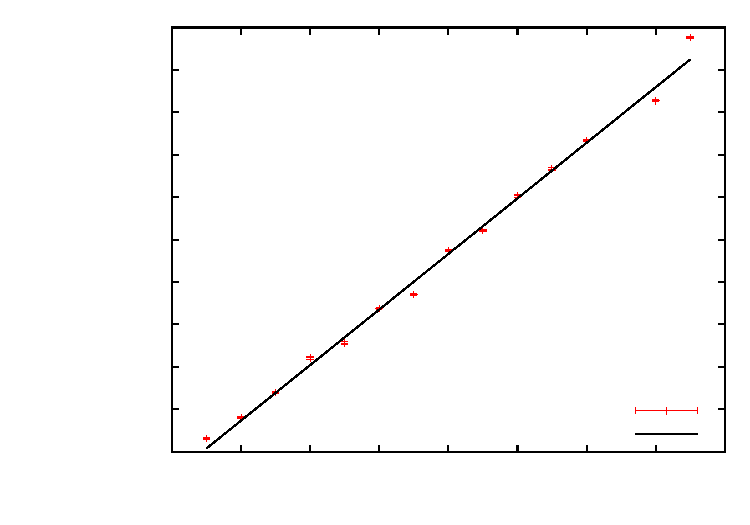
\includegraphics{gitter_reg}}%
    \gplfronttext
  \end{picture}%
\endgroup

	\caption{Gitter}
\end{figure}

\begin{table}[!htb]
	\centering
	\begin{tabular}{|c|c||c||c|c||c|c|}
		\hline
		 & & & tatsächliche &  & beste &  \\
		Objekt & Angabe & Größe [$\mu$m] & Größe [$\mu$m] & Abweichung & Größe [$\mu$m] & Abweichung \\
		\hline
		\hline
		Spalt & $B$ & $216.1 \pm 0.8$ & 250 & $14\%$ & 225 & $4\%$ \\
		Steg & $B$ & $192.2 \pm 0.6$ & 200 & $4\%$ & 195 & $2\%$ \\
		Loch & $D$ & $191.1 \pm 0.4$ & 200 & $5\%$ & - & - \\
		\hline
		Doppelloch & $B$ & $486 \pm 8$ & 500 & $3\%$ & 490 & $1\%$ \\
		(nah) & $D$ & $189 \pm 19$ & 200 & $6\%$ & 210 & $10\%$ \\
		\hline
		Doppelloch & $B$& $930 \pm 11$ & 700 & $33\%$ & 1000 & $7\%$ \\
		(mittel) & $D$& $199 \pm 21$ & 200 & $1\%$ & 210 & $6\%$ \\
		\hline		
		Gitter & $a$ & $483  \pm 11$ & 285 & $70\%$ & 490 & $2\%$ \\
		& $B$ & $194 \pm 25$ & 175 & $11\%$ & 210 & $14\%$ \\
		\hline
	\end{tabular}
\end{table}

\subsection{Wellenlänge des Lasers bestimmen}
\begin{align}
	\lambda&=mD\,,\\
	\sigma_\lambda&=D\cdot\sigma_m\,.
\end{align}


\section{Diskussion}
\label{sec:diskussion}

\section{Anhang}
\subsection{Messwerte}
\begin{figure}[!htb]
	\centering
	% GNUPLOT: LaTeX picture with Postscript
\begingroup
  \makeatletter
  \providecommand\color[2][]{%
    \GenericError{(gnuplot) \space\space\space\@spaces}{%
      Package color not loaded in conjunction with
      terminal option `colourtext'%
    }{See the gnuplot documentation for explanation.%
    }{Either use 'blacktext' in gnuplot or load the package
      color.sty in LaTeX.}%
    \renewcommand\color[2][]{}%
  }%
  \providecommand\includegraphics[2][]{%
    \GenericError{(gnuplot) \space\space\space\@spaces}{%
      Package graphicx or graphics not loaded%
    }{See the gnuplot documentation for explanation.%
    }{The gnuplot epslatex terminal needs graphicx.sty or graphics.sty.}%
    \renewcommand\includegraphics[2][]{}%
  }%
  \providecommand\rotatebox[2]{#2}%
  \@ifundefined{ifGPcolor}{%
    \newif\ifGPcolor
    \GPcolortrue
  }{}%
  \@ifundefined{ifGPblacktext}{%
    \newif\ifGPblacktext
    \GPblacktexttrue
  }{}%
  % define a \g@addto@macro without @ in the name:
  \let\gplgaddtomacro\g@addto@macro
  % define empty templates for all commands taking text:
  \gdef\gplbacktext{}%
  \gdef\gplfronttext{}%
  \makeatother
  \ifGPblacktext
    % no textcolor at all
    \def\colorrgb#1{}%
    \def\colorgray#1{}%
  \else
    % gray or color?
    \ifGPcolor
      \def\colorrgb#1{\color[rgb]{#1}}%
      \def\colorgray#1{\color[gray]{#1}}%
      \expandafter\def\csname LTw\endcsname{\color{white}}%
      \expandafter\def\csname LTb\endcsname{\color{black}}%
      \expandafter\def\csname LTa\endcsname{\color{black}}%
      \expandafter\def\csname LT0\endcsname{\color[rgb]{1,0,0}}%
      \expandafter\def\csname LT1\endcsname{\color[rgb]{0,1,0}}%
      \expandafter\def\csname LT2\endcsname{\color[rgb]{0,0,1}}%
      \expandafter\def\csname LT3\endcsname{\color[rgb]{1,0,1}}%
      \expandafter\def\csname LT4\endcsname{\color[rgb]{0,1,1}}%
      \expandafter\def\csname LT5\endcsname{\color[rgb]{1,1,0}}%
      \expandafter\def\csname LT6\endcsname{\color[rgb]{0,0,0}}%
      \expandafter\def\csname LT7\endcsname{\color[rgb]{1,0.3,0}}%
      \expandafter\def\csname LT8\endcsname{\color[rgb]{0.5,0.5,0.5}}%
    \else
      % gray
      \def\colorrgb#1{\color{black}}%
      \def\colorgray#1{\color[gray]{#1}}%
      \expandafter\def\csname LTw\endcsname{\color{white}}%
      \expandafter\def\csname LTb\endcsname{\color{black}}%
      \expandafter\def\csname LTa\endcsname{\color{black}}%
      \expandafter\def\csname LT0\endcsname{\color{black}}%
      \expandafter\def\csname LT1\endcsname{\color{black}}%
      \expandafter\def\csname LT2\endcsname{\color{black}}%
      \expandafter\def\csname LT3\endcsname{\color{black}}%
      \expandafter\def\csname LT4\endcsname{\color{black}}%
      \expandafter\def\csname LT5\endcsname{\color{black}}%
      \expandafter\def\csname LT6\endcsname{\color{black}}%
      \expandafter\def\csname LT7\endcsname{\color{black}}%
      \expandafter\def\csname LT8\endcsname{\color{black}}%
    \fi
  \fi
  \setlength{\unitlength}{0.0500bp}%
  \begin{picture}(7200.00,5040.00)%
    \gplgaddtomacro\gplbacktext{%
      \csname LTb\endcsname%
      \put(1078,704){\makebox(0,0)[r]{\strut{} 0}}%
      \put(1078,1156){\makebox(0,0)[r]{\strut{} 0.05}}%
      \put(1078,1609){\makebox(0,0)[r]{\strut{} 0.1}}%
      \put(1078,2061){\makebox(0,0)[r]{\strut{} 0.15}}%
      \put(1078,2513){\makebox(0,0)[r]{\strut{} 0.2}}%
      \put(1078,2966){\makebox(0,0)[r]{\strut{} 0.25}}%
      \put(1078,3418){\makebox(0,0)[r]{\strut{} 0.3}}%
      \put(1078,3870){\makebox(0,0)[r]{\strut{} 0.35}}%
      \put(1078,4323){\makebox(0,0)[r]{\strut{} 0.4}}%
      \put(1078,4775){\makebox(0,0)[r]{\strut{} 0.45}}%
      \put(1210,484){\makebox(0,0){\strut{} 30}}%
      \put(1909,484){\makebox(0,0){\strut{} 35}}%
      \put(2608,484){\makebox(0,0){\strut{} 40}}%
      \put(3307,484){\makebox(0,0){\strut{} 45}}%
      \put(4007,484){\makebox(0,0){\strut{} 50}}%
      \put(4706,484){\makebox(0,0){\strut{} 55}}%
      \put(5405,484){\makebox(0,0){\strut{} 60}}%
      \put(6104,484){\makebox(0,0){\strut{} 65}}%
      \put(6803,484){\makebox(0,0){\strut{} 70}}%
      \put(176,2739){\rotatebox{-270}{\makebox(0,0){\strut{}Spannung [V]}}}%
      \put(4006,154){\makebox(0,0){\strut{}Position [mm]}}%
    }%
    \gplgaddtomacro\gplfronttext{%
      \csname LTb\endcsname%
      \put(5816,4602){\makebox(0,0)[r]{\strut{}Messwerte}}%
      \csname LTb\endcsname%
      \put(5816,4382){\makebox(0,0)[r]{\strut{}Messwerte}}%
      \csname LTb\endcsname%
      \put(5816,4162){\makebox(0,0)[r]{\strut{}Messwerte}}%
    }%
    \gplbacktext
    \put(0,0){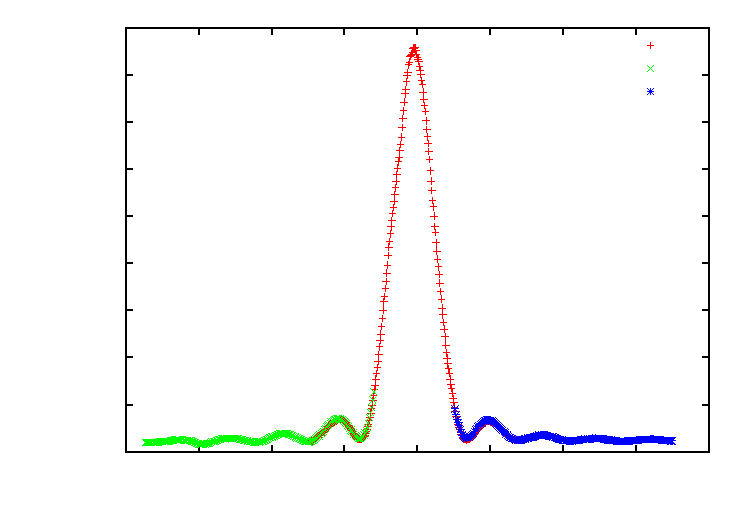
\includegraphics{spalt}}%
    \gplfronttext
  \end{picture}%
\endgroup

	\caption{Einzelspalt}
\end{figure}

\begin{figure}[!htb]
	\centering
	% GNUPLOT: LaTeX picture with Postscript
\begingroup
  \makeatletter
  \providecommand\color[2][]{%
    \GenericError{(gnuplot) \space\space\space\@spaces}{%
      Package color not loaded in conjunction with
      terminal option `colourtext'%
    }{See the gnuplot documentation for explanation.%
    }{Either use 'blacktext' in gnuplot or load the package
      color.sty in LaTeX.}%
    \renewcommand\color[2][]{}%
  }%
  \providecommand\includegraphics[2][]{%
    \GenericError{(gnuplot) \space\space\space\@spaces}{%
      Package graphicx or graphics not loaded%
    }{See the gnuplot documentation for explanation.%
    }{The gnuplot epslatex terminal needs graphicx.sty or graphics.sty.}%
    \renewcommand\includegraphics[2][]{}%
  }%
  \providecommand\rotatebox[2]{#2}%
  \@ifundefined{ifGPcolor}{%
    \newif\ifGPcolor
    \GPcolortrue
  }{}%
  \@ifundefined{ifGPblacktext}{%
    \newif\ifGPblacktext
    \GPblacktexttrue
  }{}%
  % define a \g@addto@macro without @ in the name:
  \let\gplgaddtomacro\g@addto@macro
  % define empty templates for all commands taking text:
  \gdef\gplbacktext{}%
  \gdef\gplfronttext{}%
  \makeatother
  \ifGPblacktext
    % no textcolor at all
    \def\colorrgb#1{}%
    \def\colorgray#1{}%
  \else
    % gray or color?
    \ifGPcolor
      \def\colorrgb#1{\color[rgb]{#1}}%
      \def\colorgray#1{\color[gray]{#1}}%
      \expandafter\def\csname LTw\endcsname{\color{white}}%
      \expandafter\def\csname LTb\endcsname{\color{black}}%
      \expandafter\def\csname LTa\endcsname{\color{black}}%
      \expandafter\def\csname LT0\endcsname{\color[rgb]{1,0,0}}%
      \expandafter\def\csname LT1\endcsname{\color[rgb]{0,1,0}}%
      \expandafter\def\csname LT2\endcsname{\color[rgb]{0,0,1}}%
      \expandafter\def\csname LT3\endcsname{\color[rgb]{1,0,1}}%
      \expandafter\def\csname LT4\endcsname{\color[rgb]{0,1,1}}%
      \expandafter\def\csname LT5\endcsname{\color[rgb]{1,1,0}}%
      \expandafter\def\csname LT6\endcsname{\color[rgb]{0,0,0}}%
      \expandafter\def\csname LT7\endcsname{\color[rgb]{1,0.3,0}}%
      \expandafter\def\csname LT8\endcsname{\color[rgb]{0.5,0.5,0.5}}%
    \else
      % gray
      \def\colorrgb#1{\color{black}}%
      \def\colorgray#1{\color[gray]{#1}}%
      \expandafter\def\csname LTw\endcsname{\color{white}}%
      \expandafter\def\csname LTb\endcsname{\color{black}}%
      \expandafter\def\csname LTa\endcsname{\color{black}}%
      \expandafter\def\csname LT0\endcsname{\color{black}}%
      \expandafter\def\csname LT1\endcsname{\color{black}}%
      \expandafter\def\csname LT2\endcsname{\color{black}}%
      \expandafter\def\csname LT3\endcsname{\color{black}}%
      \expandafter\def\csname LT4\endcsname{\color{black}}%
      \expandafter\def\csname LT5\endcsname{\color{black}}%
      \expandafter\def\csname LT6\endcsname{\color{black}}%
      \expandafter\def\csname LT7\endcsname{\color{black}}%
      \expandafter\def\csname LT8\endcsname{\color{black}}%
    \fi
  \fi
  \setlength{\unitlength}{0.0500bp}%
  \begin{picture}(7200.00,5040.00)%
    \gplgaddtomacro\gplbacktext{%
      \csname LTb\endcsname%
      \put(946,704){\makebox(0,0)[r]{\strut{} 0}}%
      \put(946,1383){\makebox(0,0)[r]{\strut{} 0.1}}%
      \put(946,2061){\makebox(0,0)[r]{\strut{} 0.2}}%
      \put(946,2740){\makebox(0,0)[r]{\strut{} 0.3}}%
      \put(946,3418){\makebox(0,0)[r]{\strut{} 0.4}}%
      \put(946,4097){\makebox(0,0)[r]{\strut{} 0.5}}%
      \put(946,4775){\makebox(0,0)[r]{\strut{} 0.6}}%
      \put(1078,484){\makebox(0,0){\strut{} 25}}%
      \put(1896,484){\makebox(0,0){\strut{} 30}}%
      \put(2714,484){\makebox(0,0){\strut{} 35}}%
      \put(3532,484){\makebox(0,0){\strut{} 40}}%
      \put(4349,484){\makebox(0,0){\strut{} 45}}%
      \put(5167,484){\makebox(0,0){\strut{} 50}}%
      \put(5985,484){\makebox(0,0){\strut{} 55}}%
      \put(6803,484){\makebox(0,0){\strut{} 60}}%
      \put(176,2739){\rotatebox{-270}{\makebox(0,0){\strut{}Spannung [V]}}}%
      \put(3940,154){\makebox(0,0){\strut{}Position [mm]}}%
    }%
    \gplgaddtomacro\gplfronttext{%
      \csname LTb\endcsname%
      \put(5816,4602){\makebox(0,0)[r]{\strut{}Messwerte}}%
    }%
    \gplbacktext
    \put(0,0){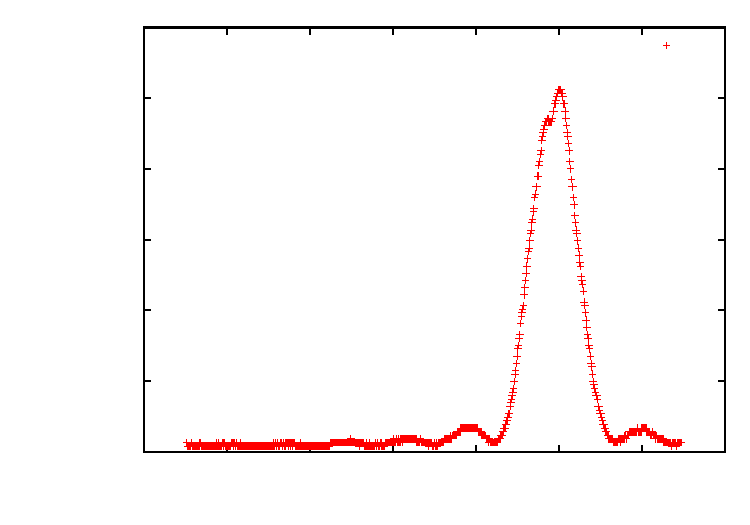
\includegraphics{spalt_grob}}%
    \gplfronttext
  \end{picture}%
\endgroup

	\caption{Einzelspalt grob}
\end{figure}

\begin{figure}[!htb]
	\centering
	% GNUPLOT: LaTeX picture with Postscript
\begingroup
  \makeatletter
  \providecommand\color[2][]{%
    \GenericError{(gnuplot) \space\space\space\@spaces}{%
      Package color not loaded in conjunction with
      terminal option `colourtext'%
    }{See the gnuplot documentation for explanation.%
    }{Either use 'blacktext' in gnuplot or load the package
      color.sty in LaTeX.}%
    \renewcommand\color[2][]{}%
  }%
  \providecommand\includegraphics[2][]{%
    \GenericError{(gnuplot) \space\space\space\@spaces}{%
      Package graphicx or graphics not loaded%
    }{See the gnuplot documentation for explanation.%
    }{The gnuplot epslatex terminal needs graphicx.sty or graphics.sty.}%
    \renewcommand\includegraphics[2][]{}%
  }%
  \providecommand\rotatebox[2]{#2}%
  \@ifundefined{ifGPcolor}{%
    \newif\ifGPcolor
    \GPcolortrue
  }{}%
  \@ifundefined{ifGPblacktext}{%
    \newif\ifGPblacktext
    \GPblacktexttrue
  }{}%
  % define a \g@addto@macro without @ in the name:
  \let\gplgaddtomacro\g@addto@macro
  % define empty templates for all commands taking text:
  \gdef\gplbacktext{}%
  \gdef\gplfronttext{}%
  \makeatother
  \ifGPblacktext
    % no textcolor at all
    \def\colorrgb#1{}%
    \def\colorgray#1{}%
  \else
    % gray or color?
    \ifGPcolor
      \def\colorrgb#1{\color[rgb]{#1}}%
      \def\colorgray#1{\color[gray]{#1}}%
      \expandafter\def\csname LTw\endcsname{\color{white}}%
      \expandafter\def\csname LTb\endcsname{\color{black}}%
      \expandafter\def\csname LTa\endcsname{\color{black}}%
      \expandafter\def\csname LT0\endcsname{\color[rgb]{1,0,0}}%
      \expandafter\def\csname LT1\endcsname{\color[rgb]{0,1,0}}%
      \expandafter\def\csname LT2\endcsname{\color[rgb]{0,0,1}}%
      \expandafter\def\csname LT3\endcsname{\color[rgb]{1,0,1}}%
      \expandafter\def\csname LT4\endcsname{\color[rgb]{0,1,1}}%
      \expandafter\def\csname LT5\endcsname{\color[rgb]{1,1,0}}%
      \expandafter\def\csname LT6\endcsname{\color[rgb]{0,0,0}}%
      \expandafter\def\csname LT7\endcsname{\color[rgb]{1,0.3,0}}%
      \expandafter\def\csname LT8\endcsname{\color[rgb]{0.5,0.5,0.5}}%
    \else
      % gray
      \def\colorrgb#1{\color{black}}%
      \def\colorgray#1{\color[gray]{#1}}%
      \expandafter\def\csname LTw\endcsname{\color{white}}%
      \expandafter\def\csname LTb\endcsname{\color{black}}%
      \expandafter\def\csname LTa\endcsname{\color{black}}%
      \expandafter\def\csname LT0\endcsname{\color{black}}%
      \expandafter\def\csname LT1\endcsname{\color{black}}%
      \expandafter\def\csname LT2\endcsname{\color{black}}%
      \expandafter\def\csname LT3\endcsname{\color{black}}%
      \expandafter\def\csname LT4\endcsname{\color{black}}%
      \expandafter\def\csname LT5\endcsname{\color{black}}%
      \expandafter\def\csname LT6\endcsname{\color{black}}%
      \expandafter\def\csname LT7\endcsname{\color{black}}%
      \expandafter\def\csname LT8\endcsname{\color{black}}%
    \fi
  \fi
  \setlength{\unitlength}{0.0500bp}%
  \begin{picture}(7200.00,5040.00)%
    \gplgaddtomacro\gplbacktext{%
      \csname LTb\endcsname%
      \put(682,704){\makebox(0,0)[r]{\strut{} 0}}%
      \put(682,1156){\makebox(0,0)[r]{\strut{} 1}}%
      \put(682,1609){\makebox(0,0)[r]{\strut{} 2}}%
      \put(682,2061){\makebox(0,0)[r]{\strut{} 3}}%
      \put(682,2513){\makebox(0,0)[r]{\strut{} 4}}%
      \put(682,2966){\makebox(0,0)[r]{\strut{} 5}}%
      \put(682,3418){\makebox(0,0)[r]{\strut{} 6}}%
      \put(682,3870){\makebox(0,0)[r]{\strut{} 7}}%
      \put(682,4323){\makebox(0,0)[r]{\strut{} 8}}%
      \put(682,4775){\makebox(0,0)[r]{\strut{} 9}}%
      \put(814,484){\makebox(0,0){\strut{} 42}}%
      \put(1563,484){\makebox(0,0){\strut{} 44}}%
      \put(2311,484){\makebox(0,0){\strut{} 46}}%
      \put(3060,484){\makebox(0,0){\strut{} 48}}%
      \put(3809,484){\makebox(0,0){\strut{} 50}}%
      \put(4557,484){\makebox(0,0){\strut{} 52}}%
      \put(5306,484){\makebox(0,0){\strut{} 54}}%
      \put(6054,484){\makebox(0,0){\strut{} 56}}%
      \put(6803,484){\makebox(0,0){\strut{} 58}}%
      \put(176,2739){\rotatebox{-270}{\makebox(0,0){\strut{}Spannung [V]}}}%
      \put(3808,154){\makebox(0,0){\strut{}Position [mm]}}%
    }%
    \gplgaddtomacro\gplfronttext{%
      \csname LTb\endcsname%
      \put(5816,4602){\makebox(0,0)[r]{\strut{}Messwerte}}%
    }%
    \gplbacktext
    \put(0,0){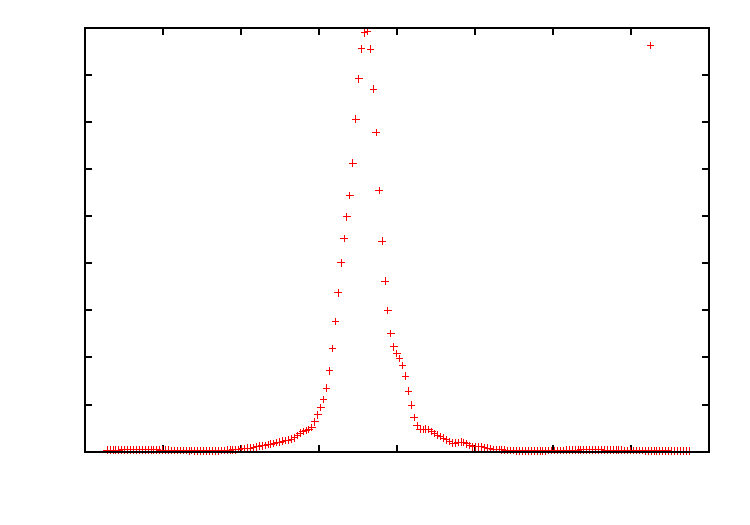
\includegraphics{steg_mitte}}%
    \gplfronttext
  \end{picture}%
\endgroup

	\caption{Steg: Hauptmaximum}
\end{figure}

\begin{figure}[!htb]
	\centering
	% GNUPLOT: LaTeX picture with Postscript
\begingroup
  \makeatletter
  \providecommand\color[2][]{%
    \GenericError{(gnuplot) \space\space\space\@spaces}{%
      Package color not loaded in conjunction with
      terminal option `colourtext'%
    }{See the gnuplot documentation for explanation.%
    }{Either use 'blacktext' in gnuplot or load the package
      color.sty in LaTeX.}%
    \renewcommand\color[2][]{}%
  }%
  \providecommand\includegraphics[2][]{%
    \GenericError{(gnuplot) \space\space\space\@spaces}{%
      Package graphicx or graphics not loaded%
    }{See the gnuplot documentation for explanation.%
    }{The gnuplot epslatex terminal needs graphicx.sty or graphics.sty.}%
    \renewcommand\includegraphics[2][]{}%
  }%
  \providecommand\rotatebox[2]{#2}%
  \@ifundefined{ifGPcolor}{%
    \newif\ifGPcolor
    \GPcolortrue
  }{}%
  \@ifundefined{ifGPblacktext}{%
    \newif\ifGPblacktext
    \GPblacktexttrue
  }{}%
  % define a \g@addto@macro without @ in the name:
  \let\gplgaddtomacro\g@addto@macro
  % define empty templates for all commands taking text:
  \gdef\gplbacktext{}%
  \gdef\gplfronttext{}%
  \makeatother
  \ifGPblacktext
    % no textcolor at all
    \def\colorrgb#1{}%
    \def\colorgray#1{}%
  \else
    % gray or color?
    \ifGPcolor
      \def\colorrgb#1{\color[rgb]{#1}}%
      \def\colorgray#1{\color[gray]{#1}}%
      \expandafter\def\csname LTw\endcsname{\color{white}}%
      \expandafter\def\csname LTb\endcsname{\color{black}}%
      \expandafter\def\csname LTa\endcsname{\color{black}}%
      \expandafter\def\csname LT0\endcsname{\color[rgb]{1,0,0}}%
      \expandafter\def\csname LT1\endcsname{\color[rgb]{0,1,0}}%
      \expandafter\def\csname LT2\endcsname{\color[rgb]{0,0,1}}%
      \expandafter\def\csname LT3\endcsname{\color[rgb]{1,0,1}}%
      \expandafter\def\csname LT4\endcsname{\color[rgb]{0,1,1}}%
      \expandafter\def\csname LT5\endcsname{\color[rgb]{1,1,0}}%
      \expandafter\def\csname LT6\endcsname{\color[rgb]{0,0,0}}%
      \expandafter\def\csname LT7\endcsname{\color[rgb]{1,0.3,0}}%
      \expandafter\def\csname LT8\endcsname{\color[rgb]{0.5,0.5,0.5}}%
    \else
      % gray
      \def\colorrgb#1{\color{black}}%
      \def\colorgray#1{\color[gray]{#1}}%
      \expandafter\def\csname LTw\endcsname{\color{white}}%
      \expandafter\def\csname LTb\endcsname{\color{black}}%
      \expandafter\def\csname LTa\endcsname{\color{black}}%
      \expandafter\def\csname LT0\endcsname{\color{black}}%
      \expandafter\def\csname LT1\endcsname{\color{black}}%
      \expandafter\def\csname LT2\endcsname{\color{black}}%
      \expandafter\def\csname LT3\endcsname{\color{black}}%
      \expandafter\def\csname LT4\endcsname{\color{black}}%
      \expandafter\def\csname LT5\endcsname{\color{black}}%
      \expandafter\def\csname LT6\endcsname{\color{black}}%
      \expandafter\def\csname LT7\endcsname{\color{black}}%
      \expandafter\def\csname LT8\endcsname{\color{black}}%
    \fi
  \fi
  \setlength{\unitlength}{0.0500bp}%
  \begin{picture}(7200.00,5040.00)%
    \gplgaddtomacro\gplbacktext{%
      \csname LTb\endcsname%
      \put(946,704){\makebox(0,0)[r]{\strut{} 0}}%
      \put(946,1383){\makebox(0,0)[r]{\strut{} 0.2}}%
      \put(946,2061){\makebox(0,0)[r]{\strut{} 0.4}}%
      \put(946,2740){\makebox(0,0)[r]{\strut{} 0.6}}%
      \put(946,3418){\makebox(0,0)[r]{\strut{} 0.8}}%
      \put(946,4097){\makebox(0,0)[r]{\strut{} 1}}%
      \put(946,4775){\makebox(0,0)[r]{\strut{} 1.2}}%
      \put(1078,484){\makebox(0,0){\strut{} 30}}%
      \put(1794,484){\makebox(0,0){\strut{} 35}}%
      \put(2509,484){\makebox(0,0){\strut{} 40}}%
      \put(3225,484){\makebox(0,0){\strut{} 45}}%
      \put(3941,484){\makebox(0,0){\strut{} 50}}%
      \put(4656,484){\makebox(0,0){\strut{} 55}}%
      \put(5372,484){\makebox(0,0){\strut{} 60}}%
      \put(6087,484){\makebox(0,0){\strut{} 65}}%
      \put(6803,484){\makebox(0,0){\strut{} 70}}%
      \put(176,2739){\rotatebox{-270}{\makebox(0,0){\strut{}Spannung [V]}}}%
      \put(3940,154){\makebox(0,0){\strut{}Position [mm]}}%
    }%
    \gplgaddtomacro\gplfronttext{%
      \csname LTb\endcsname%
      \put(5816,4602){\makebox(0,0)[r]{\strut{}Messwerte}}%
      \csname LTb\endcsname%
      \put(5816,4382){\makebox(0,0)[r]{\strut{}Messwerte}}%
      \csname LTb\endcsname%
      \put(5816,4162){\makebox(0,0)[r]{\strut{}Messwerte}}%
    }%
    \gplbacktext
    \put(0,0){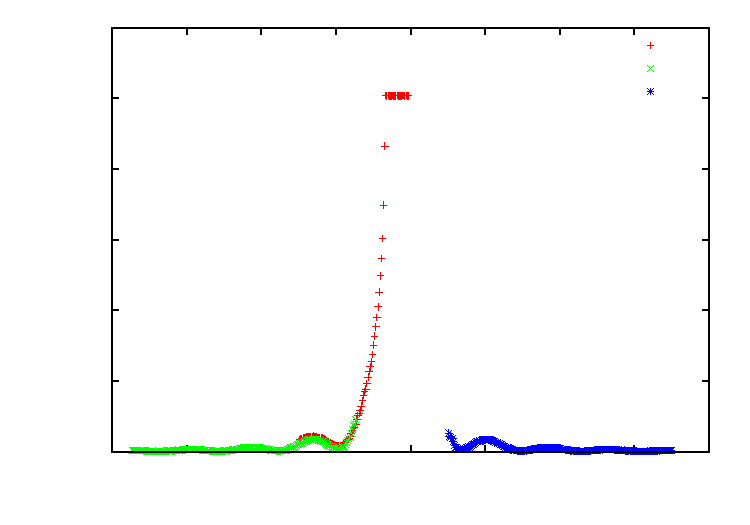
\includegraphics{steg}}%
    \gplfronttext
  \end{picture}%
\endgroup

	\caption{Steg}
\end{figure}

\begin{figure}[!htb]
	\centering
	% GNUPLOT: LaTeX picture with Postscript
\begingroup
  \makeatletter
  \providecommand\color[2][]{%
    \GenericError{(gnuplot) \space\space\space\@spaces}{%
      Package color not loaded in conjunction with
      terminal option `colourtext'%
    }{See the gnuplot documentation for explanation.%
    }{Either use 'blacktext' in gnuplot or load the package
      color.sty in LaTeX.}%
    \renewcommand\color[2][]{}%
  }%
  \providecommand\includegraphics[2][]{%
    \GenericError{(gnuplot) \space\space\space\@spaces}{%
      Package graphicx or graphics not loaded%
    }{See the gnuplot documentation for explanation.%
    }{The gnuplot epslatex terminal needs graphicx.sty or graphics.sty.}%
    \renewcommand\includegraphics[2][]{}%
  }%
  \providecommand\rotatebox[2]{#2}%
  \@ifundefined{ifGPcolor}{%
    \newif\ifGPcolor
    \GPcolortrue
  }{}%
  \@ifundefined{ifGPblacktext}{%
    \newif\ifGPblacktext
    \GPblacktexttrue
  }{}%
  % define a \g@addto@macro without @ in the name:
  \let\gplgaddtomacro\g@addto@macro
  % define empty templates for all commands taking text:
  \gdef\gplbacktext{}%
  \gdef\gplfronttext{}%
  \makeatother
  \ifGPblacktext
    % no textcolor at all
    \def\colorrgb#1{}%
    \def\colorgray#1{}%
  \else
    % gray or color?
    \ifGPcolor
      \def\colorrgb#1{\color[rgb]{#1}}%
      \def\colorgray#1{\color[gray]{#1}}%
      \expandafter\def\csname LTw\endcsname{\color{white}}%
      \expandafter\def\csname LTb\endcsname{\color{black}}%
      \expandafter\def\csname LTa\endcsname{\color{black}}%
      \expandafter\def\csname LT0\endcsname{\color[rgb]{1,0,0}}%
      \expandafter\def\csname LT1\endcsname{\color[rgb]{0,1,0}}%
      \expandafter\def\csname LT2\endcsname{\color[rgb]{0,0,1}}%
      \expandafter\def\csname LT3\endcsname{\color[rgb]{1,0,1}}%
      \expandafter\def\csname LT4\endcsname{\color[rgb]{0,1,1}}%
      \expandafter\def\csname LT5\endcsname{\color[rgb]{1,1,0}}%
      \expandafter\def\csname LT6\endcsname{\color[rgb]{0,0,0}}%
      \expandafter\def\csname LT7\endcsname{\color[rgb]{1,0.3,0}}%
      \expandafter\def\csname LT8\endcsname{\color[rgb]{0.5,0.5,0.5}}%
    \else
      % gray
      \def\colorrgb#1{\color{black}}%
      \def\colorgray#1{\color[gray]{#1}}%
      \expandafter\def\csname LTw\endcsname{\color{white}}%
      \expandafter\def\csname LTb\endcsname{\color{black}}%
      \expandafter\def\csname LTa\endcsname{\color{black}}%
      \expandafter\def\csname LT0\endcsname{\color{black}}%
      \expandafter\def\csname LT1\endcsname{\color{black}}%
      \expandafter\def\csname LT2\endcsname{\color{black}}%
      \expandafter\def\csname LT3\endcsname{\color{black}}%
      \expandafter\def\csname LT4\endcsname{\color{black}}%
      \expandafter\def\csname LT5\endcsname{\color{black}}%
      \expandafter\def\csname LT6\endcsname{\color{black}}%
      \expandafter\def\csname LT7\endcsname{\color{black}}%
      \expandafter\def\csname LT8\endcsname{\color{black}}%
    \fi
  \fi
  \setlength{\unitlength}{0.0500bp}%
  \begin{picture}(7200.00,5040.00)%
    \gplgaddtomacro\gplbacktext{%
      \csname LTb\endcsname%
      \put(1078,704){\makebox(0,0)[r]{\strut{} 0}}%
      \put(1078,1213){\makebox(0,0)[r]{\strut{} 0.01}}%
      \put(1078,1722){\makebox(0,0)[r]{\strut{} 0.02}}%
      \put(1078,2231){\makebox(0,0)[r]{\strut{} 0.03}}%
      \put(1078,2740){\makebox(0,0)[r]{\strut{} 0.04}}%
      \put(1078,3248){\makebox(0,0)[r]{\strut{} 0.05}}%
      \put(1078,3757){\makebox(0,0)[r]{\strut{} 0.06}}%
      \put(1078,4266){\makebox(0,0)[r]{\strut{} 0.07}}%
      \put(1078,4775){\makebox(0,0)[r]{\strut{} 0.08}}%
      \put(1210,484){\makebox(0,0){\strut{} 30}}%
      \put(1909,484){\makebox(0,0){\strut{} 35}}%
      \put(2608,484){\makebox(0,0){\strut{} 40}}%
      \put(3307,484){\makebox(0,0){\strut{} 45}}%
      \put(4007,484){\makebox(0,0){\strut{} 50}}%
      \put(4706,484){\makebox(0,0){\strut{} 55}}%
      \put(5405,484){\makebox(0,0){\strut{} 60}}%
      \put(6104,484){\makebox(0,0){\strut{} 65}}%
      \put(6803,484){\makebox(0,0){\strut{} 70}}%
      \put(176,2739){\rotatebox{-270}{\makebox(0,0){\strut{}Spannung [V]}}}%
      \put(4006,154){\makebox(0,0){\strut{}Position [mm]}}%
    }%
    \gplgaddtomacro\gplfronttext{%
      \csname LTb\endcsname%
      \put(5816,4602){\makebox(0,0)[r]{\strut{}Messwerte}}%
    }%
    \gplbacktext
    \put(0,0){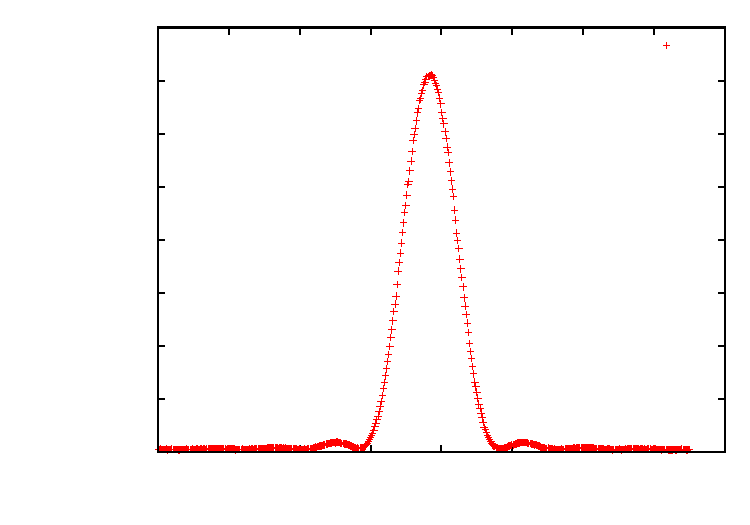
\includegraphics{loch}}%
    \gplfronttext
  \end{picture}%
\endgroup

	\caption{Lochblende}
\end{figure}

\begin{figure}[!htb]
	\centering
	% GNUPLOT: LaTeX picture with Postscript
\begingroup
  \makeatletter
  \providecommand\color[2][]{%
    \GenericError{(gnuplot) \space\space\space\@spaces}{%
      Package color not loaded in conjunction with
      terminal option `colourtext'%
    }{See the gnuplot documentation for explanation.%
    }{Either use 'blacktext' in gnuplot or load the package
      color.sty in LaTeX.}%
    \renewcommand\color[2][]{}%
  }%
  \providecommand\includegraphics[2][]{%
    \GenericError{(gnuplot) \space\space\space\@spaces}{%
      Package graphicx or graphics not loaded%
    }{See the gnuplot documentation for explanation.%
    }{The gnuplot epslatex terminal needs graphicx.sty or graphics.sty.}%
    \renewcommand\includegraphics[2][]{}%
  }%
  \providecommand\rotatebox[2]{#2}%
  \@ifundefined{ifGPcolor}{%
    \newif\ifGPcolor
    \GPcolortrue
  }{}%
  \@ifundefined{ifGPblacktext}{%
    \newif\ifGPblacktext
    \GPblacktexttrue
  }{}%
  % define a \g@addto@macro without @ in the name:
  \let\gplgaddtomacro\g@addto@macro
  % define empty templates for all commands taking text:
  \gdef\gplbacktext{}%
  \gdef\gplfronttext{}%
  \makeatother
  \ifGPblacktext
    % no textcolor at all
    \def\colorrgb#1{}%
    \def\colorgray#1{}%
  \else
    % gray or color?
    \ifGPcolor
      \def\colorrgb#1{\color[rgb]{#1}}%
      \def\colorgray#1{\color[gray]{#1}}%
      \expandafter\def\csname LTw\endcsname{\color{white}}%
      \expandafter\def\csname LTb\endcsname{\color{black}}%
      \expandafter\def\csname LTa\endcsname{\color{black}}%
      \expandafter\def\csname LT0\endcsname{\color[rgb]{1,0,0}}%
      \expandafter\def\csname LT1\endcsname{\color[rgb]{0,1,0}}%
      \expandafter\def\csname LT2\endcsname{\color[rgb]{0,0,1}}%
      \expandafter\def\csname LT3\endcsname{\color[rgb]{1,0,1}}%
      \expandafter\def\csname LT4\endcsname{\color[rgb]{0,1,1}}%
      \expandafter\def\csname LT5\endcsname{\color[rgb]{1,1,0}}%
      \expandafter\def\csname LT6\endcsname{\color[rgb]{0,0,0}}%
      \expandafter\def\csname LT7\endcsname{\color[rgb]{1,0.3,0}}%
      \expandafter\def\csname LT8\endcsname{\color[rgb]{0.5,0.5,0.5}}%
    \else
      % gray
      \def\colorrgb#1{\color{black}}%
      \def\colorgray#1{\color[gray]{#1}}%
      \expandafter\def\csname LTw\endcsname{\color{white}}%
      \expandafter\def\csname LTb\endcsname{\color{black}}%
      \expandafter\def\csname LTa\endcsname{\color{black}}%
      \expandafter\def\csname LT0\endcsname{\color{black}}%
      \expandafter\def\csname LT1\endcsname{\color{black}}%
      \expandafter\def\csname LT2\endcsname{\color{black}}%
      \expandafter\def\csname LT3\endcsname{\color{black}}%
      \expandafter\def\csname LT4\endcsname{\color{black}}%
      \expandafter\def\csname LT5\endcsname{\color{black}}%
      \expandafter\def\csname LT6\endcsname{\color{black}}%
      \expandafter\def\csname LT7\endcsname{\color{black}}%
      \expandafter\def\csname LT8\endcsname{\color{black}}%
    \fi
  \fi
  \setlength{\unitlength}{0.0500bp}%
  \begin{picture}(7200.00,5040.00)%
    \gplgaddtomacro\gplbacktext{%
      \csname LTb\endcsname%
      \put(1078,704){\makebox(0,0)[r]{\strut{} 0}}%
      \put(1078,1518){\makebox(0,0)[r]{\strut{} 0.05}}%
      \put(1078,2332){\makebox(0,0)[r]{\strut{} 0.1}}%
      \put(1078,3147){\makebox(0,0)[r]{\strut{} 0.15}}%
      \put(1078,3961){\makebox(0,0)[r]{\strut{} 0.2}}%
      \put(1078,4775){\makebox(0,0)[r]{\strut{} 0.25}}%
      \put(1210,484){\makebox(0,0){\strut{} 40}}%
      \put(1769,484){\makebox(0,0){\strut{} 42}}%
      \put(2329,484){\makebox(0,0){\strut{} 44}}%
      \put(2888,484){\makebox(0,0){\strut{} 46}}%
      \put(3447,484){\makebox(0,0){\strut{} 48}}%
      \put(4007,484){\makebox(0,0){\strut{} 50}}%
      \put(4566,484){\makebox(0,0){\strut{} 52}}%
      \put(5125,484){\makebox(0,0){\strut{} 54}}%
      \put(5684,484){\makebox(0,0){\strut{} 56}}%
      \put(6244,484){\makebox(0,0){\strut{} 58}}%
      \put(6803,484){\makebox(0,0){\strut{} 60}}%
      \put(176,2739){\rotatebox{-270}{\makebox(0,0){\strut{}Spannung [V]}}}%
      \put(4006,154){\makebox(0,0){\strut{}Position [mm]}}%
    }%
    \gplgaddtomacro\gplfronttext{%
      \csname LTb\endcsname%
      \put(5816,4602){\makebox(0,0)[r]{\strut{}Messwerte}}%
      \csname LTb\endcsname%
      \put(5816,4382){\makebox(0,0)[r]{\strut{}Messwerte}}%
      \csname LTb\endcsname%
      \put(5816,4162){\makebox(0,0)[r]{\strut{}Messwerte}}%
    }%
    \gplbacktext
    \put(0,0){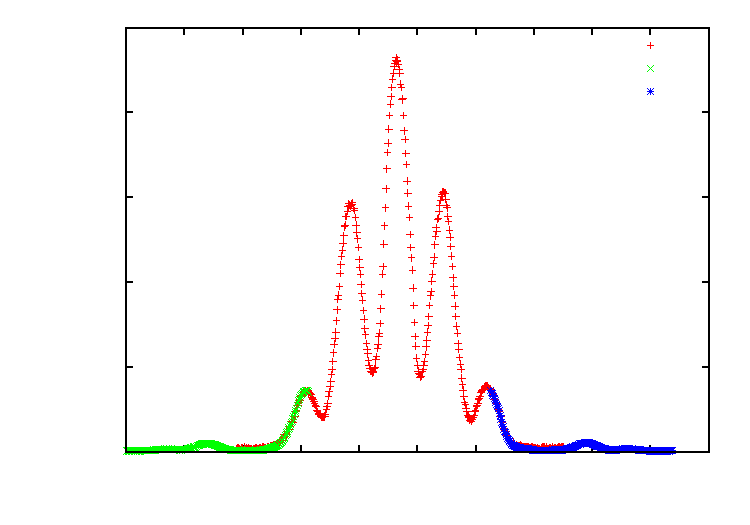
\includegraphics{doppelloch1}}%
    \gplfronttext
  \end{picture}%
\endgroup

	\caption{Doppellochblende mit dem kleinsten Lochabstand}
\end{figure}

\begin{figure}[!htb]
	\centering
	% GNUPLOT: LaTeX picture with Postscript
\begingroup
  \makeatletter
  \providecommand\color[2][]{%
    \GenericError{(gnuplot) \space\space\space\@spaces}{%
      Package color not loaded in conjunction with
      terminal option `colourtext'%
    }{See the gnuplot documentation for explanation.%
    }{Either use 'blacktext' in gnuplot or load the package
      color.sty in LaTeX.}%
    \renewcommand\color[2][]{}%
  }%
  \providecommand\includegraphics[2][]{%
    \GenericError{(gnuplot) \space\space\space\@spaces}{%
      Package graphicx or graphics not loaded%
    }{See the gnuplot documentation for explanation.%
    }{The gnuplot epslatex terminal needs graphicx.sty or graphics.sty.}%
    \renewcommand\includegraphics[2][]{}%
  }%
  \providecommand\rotatebox[2]{#2}%
  \@ifundefined{ifGPcolor}{%
    \newif\ifGPcolor
    \GPcolortrue
  }{}%
  \@ifundefined{ifGPblacktext}{%
    \newif\ifGPblacktext
    \GPblacktexttrue
  }{}%
  % define a \g@addto@macro without @ in the name:
  \let\gplgaddtomacro\g@addto@macro
  % define empty templates for all commands taking text:
  \gdef\gplbacktext{}%
  \gdef\gplfronttext{}%
  \makeatother
  \ifGPblacktext
    % no textcolor at all
    \def\colorrgb#1{}%
    \def\colorgray#1{}%
  \else
    % gray or color?
    \ifGPcolor
      \def\colorrgb#1{\color[rgb]{#1}}%
      \def\colorgray#1{\color[gray]{#1}}%
      \expandafter\def\csname LTw\endcsname{\color{white}}%
      \expandafter\def\csname LTb\endcsname{\color{black}}%
      \expandafter\def\csname LTa\endcsname{\color{black}}%
      \expandafter\def\csname LT0\endcsname{\color[rgb]{1,0,0}}%
      \expandafter\def\csname LT1\endcsname{\color[rgb]{0,1,0}}%
      \expandafter\def\csname LT2\endcsname{\color[rgb]{0,0,1}}%
      \expandafter\def\csname LT3\endcsname{\color[rgb]{1,0,1}}%
      \expandafter\def\csname LT4\endcsname{\color[rgb]{0,1,1}}%
      \expandafter\def\csname LT5\endcsname{\color[rgb]{1,1,0}}%
      \expandafter\def\csname LT6\endcsname{\color[rgb]{0,0,0}}%
      \expandafter\def\csname LT7\endcsname{\color[rgb]{1,0.3,0}}%
      \expandafter\def\csname LT8\endcsname{\color[rgb]{0.5,0.5,0.5}}%
    \else
      % gray
      \def\colorrgb#1{\color{black}}%
      \def\colorgray#1{\color[gray]{#1}}%
      \expandafter\def\csname LTw\endcsname{\color{white}}%
      \expandafter\def\csname LTb\endcsname{\color{black}}%
      \expandafter\def\csname LTa\endcsname{\color{black}}%
      \expandafter\def\csname LT0\endcsname{\color{black}}%
      \expandafter\def\csname LT1\endcsname{\color{black}}%
      \expandafter\def\csname LT2\endcsname{\color{black}}%
      \expandafter\def\csname LT3\endcsname{\color{black}}%
      \expandafter\def\csname LT4\endcsname{\color{black}}%
      \expandafter\def\csname LT5\endcsname{\color{black}}%
      \expandafter\def\csname LT6\endcsname{\color{black}}%
      \expandafter\def\csname LT7\endcsname{\color{black}}%
      \expandafter\def\csname LT8\endcsname{\color{black}}%
    \fi
  \fi
  \setlength{\unitlength}{0.0500bp}%
  \begin{picture}(7200.00,5040.00)%
    \gplgaddtomacro\gplbacktext{%
      \csname LTb\endcsname%
      \put(1078,704){\makebox(0,0)[r]{\strut{} 0}}%
      \put(1078,1213){\makebox(0,0)[r]{\strut{} 0.02}}%
      \put(1078,1722){\makebox(0,0)[r]{\strut{} 0.04}}%
      \put(1078,2231){\makebox(0,0)[r]{\strut{} 0.06}}%
      \put(1078,2740){\makebox(0,0)[r]{\strut{} 0.08}}%
      \put(1078,3248){\makebox(0,0)[r]{\strut{} 0.1}}%
      \put(1078,3757){\makebox(0,0)[r]{\strut{} 0.12}}%
      \put(1078,4266){\makebox(0,0)[r]{\strut{} 0.14}}%
      \put(1078,4775){\makebox(0,0)[r]{\strut{} 0.16}}%
      \put(1210,484){\makebox(0,0){\strut{} 42}}%
      \put(1909,484){\makebox(0,0){\strut{} 44}}%
      \put(2608,484){\makebox(0,0){\strut{} 46}}%
      \put(3307,484){\makebox(0,0){\strut{} 48}}%
      \put(4007,484){\makebox(0,0){\strut{} 50}}%
      \put(4706,484){\makebox(0,0){\strut{} 52}}%
      \put(5405,484){\makebox(0,0){\strut{} 54}}%
      \put(6104,484){\makebox(0,0){\strut{} 56}}%
      \put(6803,484){\makebox(0,0){\strut{} 58}}%
      \put(176,2739){\rotatebox{-270}{\makebox(0,0){\strut{}Spannung [V]}}}%
      \put(4006,154){\makebox(0,0){\strut{}Position [mm]}}%
    }%
    \gplgaddtomacro\gplfronttext{%
      \csname LTb\endcsname%
      \put(5816,4602){\makebox(0,0)[r]{\strut{}Messwerte}}%
    }%
    \gplbacktext
    \put(0,0){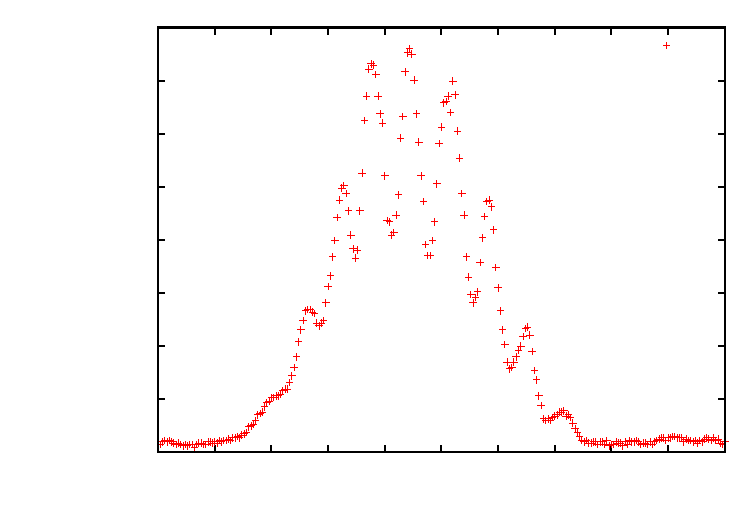
\includegraphics{doppelloch2}}%
    \gplfronttext
  \end{picture}%
\endgroup

	\caption{Doppellochblende mit dem mittleren Lochabstand}
\end{figure}

\begin{figure}[!htb]
	\centering
	% GNUPLOT: LaTeX picture with Postscript
\begingroup
  \makeatletter
  \providecommand\color[2][]{%
    \GenericError{(gnuplot) \space\space\space\@spaces}{%
      Package color not loaded in conjunction with
      terminal option `colourtext'%
    }{See the gnuplot documentation for explanation.%
    }{Either use 'blacktext' in gnuplot or load the package
      color.sty in LaTeX.}%
    \renewcommand\color[2][]{}%
  }%
  \providecommand\includegraphics[2][]{%
    \GenericError{(gnuplot) \space\space\space\@spaces}{%
      Package graphicx or graphics not loaded%
    }{See the gnuplot documentation for explanation.%
    }{The gnuplot epslatex terminal needs graphicx.sty or graphics.sty.}%
    \renewcommand\includegraphics[2][]{}%
  }%
  \providecommand\rotatebox[2]{#2}%
  \@ifundefined{ifGPcolor}{%
    \newif\ifGPcolor
    \GPcolortrue
  }{}%
  \@ifundefined{ifGPblacktext}{%
    \newif\ifGPblacktext
    \GPblacktexttrue
  }{}%
  % define a \g@addto@macro without @ in the name:
  \let\gplgaddtomacro\g@addto@macro
  % define empty templates for all commands taking text:
  \gdef\gplbacktext{}%
  \gdef\gplfronttext{}%
  \makeatother
  \ifGPblacktext
    % no textcolor at all
    \def\colorrgb#1{}%
    \def\colorgray#1{}%
  \else
    % gray or color?
    \ifGPcolor
      \def\colorrgb#1{\color[rgb]{#1}}%
      \def\colorgray#1{\color[gray]{#1}}%
      \expandafter\def\csname LTw\endcsname{\color{white}}%
      \expandafter\def\csname LTb\endcsname{\color{black}}%
      \expandafter\def\csname LTa\endcsname{\color{black}}%
      \expandafter\def\csname LT0\endcsname{\color[rgb]{1,0,0}}%
      \expandafter\def\csname LT1\endcsname{\color[rgb]{0,1,0}}%
      \expandafter\def\csname LT2\endcsname{\color[rgb]{0,0,1}}%
      \expandafter\def\csname LT3\endcsname{\color[rgb]{1,0,1}}%
      \expandafter\def\csname LT4\endcsname{\color[rgb]{0,1,1}}%
      \expandafter\def\csname LT5\endcsname{\color[rgb]{1,1,0}}%
      \expandafter\def\csname LT6\endcsname{\color[rgb]{0,0,0}}%
      \expandafter\def\csname LT7\endcsname{\color[rgb]{1,0.3,0}}%
      \expandafter\def\csname LT8\endcsname{\color[rgb]{0.5,0.5,0.5}}%
    \else
      % gray
      \def\colorrgb#1{\color{black}}%
      \def\colorgray#1{\color[gray]{#1}}%
      \expandafter\def\csname LTw\endcsname{\color{white}}%
      \expandafter\def\csname LTb\endcsname{\color{black}}%
      \expandafter\def\csname LTa\endcsname{\color{black}}%
      \expandafter\def\csname LT0\endcsname{\color{black}}%
      \expandafter\def\csname LT1\endcsname{\color{black}}%
      \expandafter\def\csname LT2\endcsname{\color{black}}%
      \expandafter\def\csname LT3\endcsname{\color{black}}%
      \expandafter\def\csname LT4\endcsname{\color{black}}%
      \expandafter\def\csname LT5\endcsname{\color{black}}%
      \expandafter\def\csname LT6\endcsname{\color{black}}%
      \expandafter\def\csname LT7\endcsname{\color{black}}%
      \expandafter\def\csname LT8\endcsname{\color{black}}%
    \fi
  \fi
  \setlength{\unitlength}{0.0500bp}%
  \begin{picture}(7200.00,5040.00)%
    \gplgaddtomacro\gplbacktext{%
      \csname LTb\endcsname%
      \put(946,704){\makebox(0,0)[r]{\strut{} 0}}%
      \put(946,1111){\makebox(0,0)[r]{\strut{} 0.2}}%
      \put(946,1518){\makebox(0,0)[r]{\strut{} 0.4}}%
      \put(946,1925){\makebox(0,0)[r]{\strut{} 0.6}}%
      \put(946,2332){\makebox(0,0)[r]{\strut{} 0.8}}%
      \put(946,2740){\makebox(0,0)[r]{\strut{} 1}}%
      \put(946,3147){\makebox(0,0)[r]{\strut{} 1.2}}%
      \put(946,3554){\makebox(0,0)[r]{\strut{} 1.4}}%
      \put(946,3961){\makebox(0,0)[r]{\strut{} 1.6}}%
      \put(946,4368){\makebox(0,0)[r]{\strut{} 1.8}}%
      \put(946,4775){\makebox(0,0)[r]{\strut{} 2}}%
      \put(1078,484){\makebox(0,0){\strut{} 40}}%
      \put(1598,484){\makebox(0,0){\strut{} 42}}%
      \put(2119,484){\makebox(0,0){\strut{} 44}}%
      \put(2639,484){\makebox(0,0){\strut{} 46}}%
      \put(3160,484){\makebox(0,0){\strut{} 48}}%
      \put(3680,484){\makebox(0,0){\strut{} 50}}%
      \put(4201,484){\makebox(0,0){\strut{} 52}}%
      \put(4721,484){\makebox(0,0){\strut{} 54}}%
      \put(5242,484){\makebox(0,0){\strut{} 56}}%
      \put(5762,484){\makebox(0,0){\strut{} 58}}%
      \put(6283,484){\makebox(0,0){\strut{} 60}}%
      \put(6803,484){\makebox(0,0){\strut{} 62}}%
      \put(176,2739){\rotatebox{-270}{\makebox(0,0){\strut{}Spannung [V]}}}%
      \put(3940,154){\makebox(0,0){\strut{}Position [mm]}}%
    }%
    \gplgaddtomacro\gplfronttext{%
      \csname LTb\endcsname%
      \put(5816,4602){\makebox(0,0)[r]{\strut{}Messwerte}}%
      \csname LTb\endcsname%
      \put(5816,4382){\makebox(0,0)[r]{\strut{}Messwerte}}%
      \csname LTb\endcsname%
      \put(5816,4162){\makebox(0,0)[r]{\strut{}Messwerte}}%
    }%
    \gplbacktext
    \put(0,0){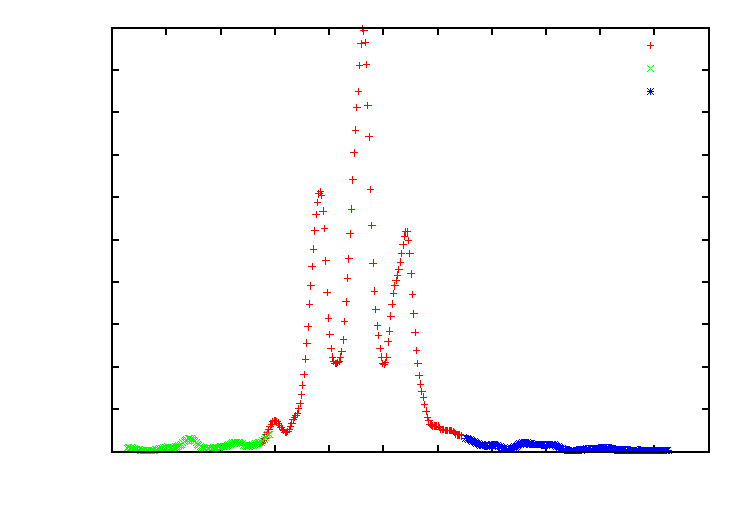
\includegraphics{gitter}}%
    \gplfronttext
  \end{picture}%
\endgroup

	\caption{Gitter}
\end{figure}

\subsection{Extrema Tabelle}
\begin{table}[!htb]
	\centering
	\begin{tabular}{|c||c|c|c|c|}
		\hline		
		Objekt & $\frac{\varepsilon}{\pi}$ & \multicolumn{2}{c}{Position [mm]} & Winkel $\alpha$ \\
		& & absolut & relativ & [$10^{-3}~$rad] \\
		\hline
		\hline
		&	-4	&	35.225	&	-14.575	&	-2.974	\\
		&	-3.5	&	37.288	&	-12.513	&	-2.554	\\
		&	-3	&	38.825	&	-10.975	&	-2.240	\\
		&	-2.5	&	40.850	&	-8.950	&	-1.827	\\
		&	-2	&	42.575	&	-7.225	&	-1.474	\\
		&	-1.5	&	44.575	&	-5.225	&	-1.066	\\
		&	-1	&	46.025	&	-3.775	&	-0.770	\\
		Spalt &	0	&	49.800	&	0.000	&	0.000	\\
		&	1	&	53.375	&	3.575	&	0.730	\\
		&	1.5	&	54.900	&	5.100	&	1.041	\\
		&	2	&	56.963	&	7.163	&	1.462	\\
		&	2.5	&	58.650	&	8.850	&	1.806	\\
		&	3	&	60.525	&	10.725	&	2.189	\\
		&	3.5	&	62.250	&	12.450	&	2.541	\\
		&	4	&	64.150	&	14.350	&	2.929	\\
		\hline
		&	-4	&	33.050	&	-16.200	&	-3.306	\\
		&	-3.5	&	35.225	&	-14.025	&	-2.862	\\
		&	-3	&	37.138	&	-12.113	&	-2.472	\\
		&	-2.5	&	39.238	&	-10.013	&	-2.043	\\
		&	-2	&	41.175	&	-8.075	&	-1.648	\\
		&	-1.5	&	43.475	&	-5.775	&	-1.179	\\
		&	-1	&	45.175	&	-4.075	&	-0.832	\\
		Steg &	0	&	49.250	&	0.000	&	0.000	\\
		&	1	&	53.400	&	4.150	&	0.847	\\
		&	1.5	&	55.088	&	5.838	&	1.191	\\
		&	2	&	57.450	&	8.200	&	1.673	\\
		&	2.5	&	59.250	&	10.000	&	2.041	\\
		&	3	&	61.425	&	12.175	&	2.485	\\
		&	3.5	&	63.300	&	14.050	&	2.867	\\
		&	4	&	65.550	&	16.300	&	3.327	\\
		\hline
		&	3.6987	&	34.125	&	-15.075	&	-3.077	\\
		&	3.2383	&	36.075	&	-13.125	&	-2.679	\\
		&	2.6793	&	38.325	&	-10.875	&	-2.219	\\
		&	2.2331	&	40.125	&	-9.075	&	-1.852	\\
		&	1.6347	&	42.600	&	-6.600	&	-1.347	\\
		&	1.2197	&	44.100	&	-5.100	&	-1.041	\\
		Loch- &	0	&	49.200	&	0.000	&	0.000	\\
		blende &	1.2197	&	54.075	&	4.875	&	0.995	\\
		&	1.6347	&	55.800	&	6.600	&	1.347	\\
		&	2.2331	&	58.350	&	9.150	&	1.867	\\
		&	2.6793	&	60.150	&	10.950	&	2.235	\\
		&	3.2383	&	62.400	&	13.200	&	2.694	\\
		&	3.6987	&	64.125	&	14.925	&	3.046	\\
		&	4.2411	&	66.250	&	17.050	&	3.480	\\
		\hline
	\end{tabular}
\end{table}

\begin{table}[!htb]
	\centering
	\begin{tabular}{|c||c|c|c|c|}
		\hline		
		Objekt & $\frac{\varepsilon}{\pi}$ & \multicolumn{2}{c}{Position [mm]} & Winkel $\alpha$ \\
		& & absolut & relativ & [$10^{-3}~$rad] \\
		\hline
		\hline
		&	-2	&	46.200	&	-3.088	&	-0.630	\\
		&	-1.5	&	46.800	&	-2.488	&	-0.508	\\
		&	-1	&	47.713	&	-1.575	&	-0.321	\\
		Doppel- &	-0.5	&	48.463	&	-0.825	&	-0.168	\\
		loch &	0	&	49.288	&	0.000	&	0.000	\\
		(nah) &	0.5	&	50.113	&	0.825	&	0.168	\\
		&	1	&	50.900	&	1.613	&	0.329	\\
		&	1.5	&	51.850	&	2.563	&	0.523	\\
		&	2	&	52.375	&	3.088	&	0.630	\\
		\hline
		&	-3	&	47.050	&	-2.250	&	-0.459	\\
		&	-2.5	&	47.300	&	-2.000	&	-0.408	\\
		&	-2	&	47.800	&	-1.500	&	-0.306	\\
		&	-1.5	&	48.100	&	-1.200	&	-0.245	\\
		&	-1	&	48.450	&	-0.850	&	-0.173	\\
		Doppel- &	-0.5	&	48.900	&	-0.400	&	-0.082	\\
		loch &	0	&	49.300	&	0.000	&	0.000	\\
		(mittel) &	0.5	&	49.725	&	0.425	&	0.087	\\
		&	1	&	50.150	&	0.850	&	0.173	\\
		&	1.5	&	50.700	&	1.400	&	0.286	\\
		&	2	&	51.050	&	1.750	&	0.357	\\
		&	2.5	&	51.500	&	2.200	&	0.449	\\
		&	3	&	51.900	&	2.600	&	0.531	\\
		&	3.5	&	52.350	&	3.050	&	0.622	\\
		&	4	&	52.775	&	3.475	&	0.709	\\
		\hline
		&	-4.5	&	42.250	&	-7.000	&	-1.429	\\
		&	-4	&	42.850	&	-6.400	&	-1.306	\\
		&	-3.5	&	43.575	&	-5.675	&	-1.158	\\
		&	-3	&	44.575	&	-4.675	&	-0.954	\\
		&	-2.5	&	45.000	&	-4.250	&	-0.867	\\
		&	-2	&	46.000	&	-3.250	&	-0.663	\\
		Gitter &	-1.5	&	46.400	&	-2.850	&	-0.582	\\
		&	-1	&	47.675	&	-1.575	&	-0.321	\\
		&	-0.5	&	48.250	&	-1.000	&	-0.204	\\
		&	0	&	49.250	&	0.000	&	0.000	\\
		&	0.5	&	50.025	&	0.775	&	0.158	\\
		&	1	&	50.850	&	1.600	&	0.327	\\
		&	1.5	&	53.825	&	4.575	&	0.934	\\
		&	2	&	52.000	&	2.750	&	0.561	\\
		&	2.5	&	53.825	&	4.575	&	0.934	\\
		\hline
	\end{tabular}
\end{table}

\bibliography{literatur}
\bibliographystyle{babalpha}

\end{document}
